\documentclass{beamer}
% \usepackage[TU]{fontenc}
\usepackage{lmodern} % load a font with all the characters
% \usepackage{unicode-math}

\setlength{\parskip}{\baselineskip} 

% Essential packages
\usepackage[english,danish]{babel}
\usepackage[utf8]{inputenc}
\usepackage{textcomp}
\usepackage[skins,minted,breakable]{tcolorbox}
\usepackage{booktabs}
\usepackage{pifont}

% Math packages
\usepackage{amsmath,amsfonts,amssymb,amsthm}
\usepackage{pgfplots}
\usepackage{pgfplotstable}

% Programming packages
\usepackage{listings,newtxtt}
\usepackage[ruled,vlined,linesnumbered]{algorithm2e}
\usepackage{courier}

% Layout packages
\usepackage{csquotes}
\usepackage{booktabs}
\usepackage{multicol}
\usepackage{graphicx}
\usepackage{fancyhdr}
\usepackage{lipsum}
\usepackage{subcaption}
\usepackage[style=numeric-comp,maxbibnames=99]{biblatex}
\usepackage{forest}
\usepackage{array}
\usepackage{colortbl}
\usepackage{outlines}

\usepackage{tikz}  
\usetikzlibrary{
    calc,
    matrix,
    chains,
    positioning,
    arrows.meta,
    bending,
    shapes.arrows,
    calc,
    positioning,
    backgrounds,
    decorations.pathreplacing,
    calligraphy,
}

\addbibresource{bibliography.bib}
\addbibresource{iacr.bib}

\newcommand{\eff}{\mathbb{F}} % Fancy F
\newcommand{\pp}{\texttt{++}} % ++ operator
\newcommand{\rightshift}{\texttt{ >> }} 
\newcommand{\td}[1]{\todo[inline]{#1}} % Todo notes
\newcommand{\cmark}{\ding{51}}%
\newcommand{\xmark}{\ding{55}}%

\title{Implementation and Evaluation of Dinur's MQ Solver Algorithm}
\author{Author: Mikkel Juul Vestergaard\\Supervisor: Associate Professor Ruben Niederhagen}
\institute{Department of Mathematics and Computer Science\\University of Southern Denmark}
\date{Thesis Defence, 2023}

\AtBeginSubsection[]
{
  \begin{frame}
    \frametitle{Table of Contents}
    \tableofcontents[sectionstyle=show/shaded,subsectionstyle=show/shaded/hide]
  \end{frame}
}

\begin{document}

\frame{\titlepage}

\section{Introduction}
\subsection{Polynomials 101}
\begin{frame}
    \frametitle{Polynomials?}
    A mathematical expression or function in some variable(s), coefficients and declared through the operators:
    \begin{itemize}
        \item Addition.
        \item Subtraction.
        \item Multiplication.
        \item Exponentiation using non-negative integers.
    \end{itemize}
\end{frame}

% \begin{frame}
%     \frametitle{Polynomials.}
%     Some simple polynomials as mathematical functions:
%     \begin{equation*}
%         \begin{split}
%             p(x) &= 4x + 1\\
%             f(x) &= 2x^2 + 3
%         \end{split}
%     \end{equation*}
%     and expressions:
%     \begin{equation*}
%         \begin{split}
%             &x^{10}\\
%             &x^5 + 10x^3
%         \end{split}
%     \end{equation*}

% \end{frame}

% \begin{frame}
%     \frametitle{Multivariate polynomials.}
%     So, what are these \textit{multivariate} polynomials?
    
%     \pause 

%     Well, just polynomials in \textit{multiple} variables!

%     \pause 

%     Typically we denote these variables by subscript (of course starting from $0$).

%     E.g. $x_0, x_1, \dots x_{n - 1}$, however, we can still of course call them $x, y, z$, etc.

%     \pause 

%     For a notational shorthand, 
%     $$
%         \mathbf{x} = (x_0, x_1, \dots x_{n - 1})
%     $$ 
%     for $n$ variables, and likewise for variables denoted by $y$s and $z$s.
% \end{frame}

% \begin{frame}
%     \frametitle{Multivariate polynomials.}
%     So how do these look?

%     \pause 

%     Quite simply, they look like the polynomials we just saw but with more variables!

%     \pause 
%     For example:
%     \begin{equation*}
%         \begin{split}
%             p_0(x_0, x_1, x_2, x_3) &= 5x_3^4 + x_0^2 + 4x_1 + 10\\
%             p_1(x_0, x_1, x_2, x_3) &= 3x_1x_2x_3 + 2x_0^2
%         \end{split}
%     \end{equation*}
% \end{frame}

\begin{frame}
    \frametitle{Boolean multivariate polynomials?}
    Polynomials as we know them, just with more variables: $x_0, x_1, \dots x_{n - 1}$ (or $x, y, z, etc.$).

    \pause 
    
    Coefficients and variable assignments may only be 0 and 1.

    \pause 

    I.e. these polynomials may look like 
    \begin{equation*}
        \begin{split}
            &x_0x_1 + x_0\\
            &x_0^2 + x_1x_2
        \end{split}
    \end{equation*}

    \pause

    For shorthand notation: $\mathbf{x} = (x_0, x_1, \dots x_{n - 1})$.

\end{frame}

\subsection{What is the ''MQ-problem''?}
\begin{frame}
    \frametitle{The MQ-problem}
    Well, the MQ-problem relates to multivariate polynomials. How so, you ask?
    \pause
    \begin{outline}
        \1 A system of multivariate polynomials.
            \2 $m$ polynomials. 
            \2 $n$ variables.
            \2 The polynomials are of degree $d$.
            \2 From this point on, systems of polynomials are written as $\mathcal{P} = \{p_0, p_1, p_2, \dots p_{m-1}\}$
    \end{outline}

    \pause 

    We typically say that a \textit{solution} to a system $\mathcal{P}$ is an assignment of the variables of the polynomial s.t. 
    $$
        p_{0}(\hat{\mathbf{x}}) = p_{1}(\hat{\mathbf{x}}) = \dots = p_{m-1}(\hat{\mathbf{x}}) = 0
    $$
\end{frame}

\begin{frame}
    \frametitle{The MQ-problem}
    All right, why bother?
    \pause
    \begin{outline}
        \1 Solving systems of multivariate polynomials (in general) is hard for a computer!
            \2 We often denote $MP$ as the problem of solving multivariate polynomials of degree $d$ in $n$ variables and $m$ polynomials.

        \pause 

        \1 A commonly used version of the $MP$-problem is the $MQ$-problem.
            \2 This is the problem of solving systems of $m$ quadratic polynomials in $n$ variables.
            \2 This is also very hard for a computer to solve while having nice properties for real implementations.
            \2 Much modern cryptography is based on the hardness of this problem.
    \end{outline}
\end{frame}

\begin{frame}
    \frametitle{So why is this problem \textit{hard}?}
    For \textit{boolean} multivariate polynomials, searching through all possible variable assignments is slow in the worst case!

    \pause 

    \begin{equation*}
        \begin{array}{cccccc}
            p(  & x_0,  & x_1,      & \dots    & x_{n - 1}                  & )\\
                & \uncover<3->{2}     & \uncover<4->{\cdot 2}   & \uncover<5->{\cdots}  & \uncover<6->{\cdot 2}  & \uncover<7->{= 2^n}
        \end{array}
    \end{equation*}
    
    \pause[8]

    $2^n$ grows quickly, making it hard for computers to work with large problem sizes.

    \pause[9]

    Can we search through \textit{fewer} than all $n$ variables to find a solution?
\end{frame}

\subsection{The algorithm}
\begin{frame}
    \frametitle{Dinur's algorithm}
    In \cite{eurocrypt-2021-30841}, Dinur proposed an algorithm for $MP$ problems with \textbf{exponential speedup} over exhaustive search.

    The algorithm is based on the \textit{polynomial-method}, which is borrowed from circuit complexity.

    To the best of my knowledge, this algorithm has not been tested in practice.

    It borrows ideas from other algorithms based on the same method.
\end{frame}

\begin{frame}
    \frametitle{The Polynomial method}
    Algorithms based on the polynomial method solve systems 
    $$
        \mathcal{P} = \{p_j(\mathbf{x})\}^{m - 1}_{j = 0}
    $$ 
    by considering constructing a polynomial 
    $$
        F(\mathbf{x}) = (1 + p_0(\mathbf{x}))(1 + p_1(\mathbf{x})) \dots (1 + p_{m - 1}(\mathbf{x}))
    $$
    with multiplication and addition acting as noted earlier.

    Also, notice how only solutions to $\mathcal{P}$ evaluate to $1$ on $F$.
\end{frame}

\begin{frame}
    \frametitle{The Polynomial method}
    However, since $F$ may have a rather high degree ($m \cdot d$), the methods may instead \textit{generate} a related system, 
    $$
        \Tilde{\mathcal{P}}_k \gets \left\{r_i(\mathbf{x}) = \sum_{j = 0}^{m-1}A_{i,j} \cdot p_j(\mathbf{x})\right\}^{\ell - 1}_{i = 0},
    $$
    with a random matrix $A$ of rank $\ell$, which allows for constructing the \textit{probabilistic polynomial}
    $$
        \Tilde{F}(\mathbf{x}) = (1 + r_0(\mathbf{x}))(1 + r_1(\mathbf{x})) \dots (1 + r_{\ell - 1}(\mathbf{x})) 
    $$
    of smaller degree ($d \cdot \ell$), assuming one chooses an $\ell < m$.
\end{frame}

\begin{frame}
    \frametitle{Isolating solutions}
    Let us consider a system with polynomials $p_0$ and $p_1$, over $6$ variables. 

    \pause
    Say we split the variables so that the first four variables are the $\mathbf{y}$-variables, and the last two variables are the $\mathbf{z}$-variables. I.e. 
    $$
        ({\color{cyan}x_0}, {\color{cyan}x_1}, {\color{cyan}x_2}, {\color{cyan}x_3}, {\color{purple}x_4}, {\color{purple}x_5}) = ({\color{cyan}y_0}, {\color{cyan}y_1}, {\color{cyan}y_2}, {\color{cyan}y_3}, {\color{purple}z_0}, {\color{purple}z_1})
    $$
    with colors denoting $\color{cyan}\mathbf{y}$-variables and $\color{purple}\mathbf{z}$-variables.
\end{frame}

\begin{frame}
    \frametitle{Isolating solutions, why?}
    Now, let us examine the following examples
    \begin{equation*}
        \begin{split}
            &p_0({\color{cyan}1}, {\color{cyan}1}, {\color{cyan}1}, {\color{cyan}0}, {\color{purple}0}, {\color{purple}0}) = 0, p_1({\color{cyan}1}, {\color{cyan}1}, {\color{cyan}1}, {\color{cyan}0}, {\color{purple}0}, {\color{purple}0}) = 0 \uncover<2->{\text{ \color{green}\cmark}}\\
            &p_0({\color{cyan}1}, {\color{cyan}1}, {\color{cyan}1}, {\color{cyan}0}, {\color{purple}0}, {\color{purple}1}) = 1, p_1({\color{cyan}1}, {\color{cyan}1}, {\color{cyan}1}, {\color{cyan}0}, {\color{purple}0}, {\color{purple}1}) = 0 \uncover<3->{\text{ \color{red}\xmark}}\\
            &p_0({\color{cyan}1}, {\color{cyan}1}, {\color{cyan}1}, {\color{cyan}0}, {\color{purple}1}, {\color{purple}0}) = 0, p_1({\color{cyan}1}, {\color{cyan}1}, {\color{cyan}1}, {\color{cyan}0}, {\color{purple}1}, {\color{purple}0}) = 1 \uncover<4->{\text{ \color{red}\xmark}}\\
            &p_0({\color{cyan}1}, {\color{cyan}1}, {\color{cyan}1}, {\color{cyan}0}, {\color{purple}1}, {\color{purple}1}) = 1, p_1({\color{cyan}1}, {\color{cyan}1}, {\color{cyan}1}, {\color{cyan}0}, {\color{purple}1}, {\color{purple}1}) = 0 \uncover<5->{\text{ \color{red}\xmark}}
        \end{split}
    \end{equation*}
    and 
    \begin{equation*}
        \begin{split}
            &p_0({\color{cyan}1}, {\color{cyan}0}, {\color{cyan}0}, {\color{cyan}1}, {\color{purple}0}, {\color{purple}0}) = 0, p_1({\color{cyan}1}, {\color{cyan}0}, {\color{cyan}0}, {\color{cyan}1}, {\color{purple}0}, {\color{purple}0}) = 0 \uncover<6->{\text{ \color{green}\cmark}}\\
            &p_0({\color{cyan}1}, {\color{cyan}0}, {\color{cyan}0}, {\color{cyan}1}, {\color{purple}0}, {\color{purple}1}) = 0, p_1({\color{cyan}1}, {\color{cyan}0}, {\color{cyan}0}, {\color{cyan}1}, {\color{purple}0}, {\color{purple}1}) = 1 \uncover<7->{\text{ \color{red}\xmark}}\\
            &p_0({\color{cyan}1}, {\color{cyan}0}, {\color{cyan}0}, {\color{cyan}1}, {\color{purple}1}, {\color{purple}0}) = 0, p_1({\color{cyan}1}, {\color{cyan}0}, {\color{cyan}0}, {\color{cyan}1}, {\color{purple}1}, {\color{purple}0}) = 0 \uncover<8->{\text{ \color{green}\cmark}}\\
            &p_0({\color{cyan}1}, {\color{cyan}0}, {\color{cyan}0}, {\color{cyan}1}, {\color{purple}1}, {\color{purple}1}) = 1, p_1({\color{cyan}1}, {\color{cyan}0}, {\color{cyan}0}, {\color{cyan}1}, {\color{purple}1}, {\color{purple}1}) = 0 \uncover<9->{\text{ \color{red}\xmark}}
        \end{split}
    \end{equation*}
\end{frame}

\begin{frame}
    \frametitle{Recovering bits}
        We can actually create the polynomials
        \begin{itemize}
            \item[] $U_0(\mathbf{y})$: Count parity of evaluations to $\tilde{F}(\mathbf{y}, \hat{\mathbf{z}})$ for all assignments of $\hat{\mathbf{z}}$.
            \vspace{0.5cm}
            \item[] $U_i(\mathbf{y})$, for $i = 1, \dots n_1$: Count parity of evaluations to $\tilde{F}(\mathbf{y}, \hat{\mathbf{z}})$ for all assignments of $\hat{\mathbf{z}}$ with $z_{i - 1} = 0$.
        \end{itemize}

        \pause

        This means that\\
        $\hat{\mathbf{y}}$ is part of an \textit{isolated solution} $\implies$ $U_0(\hat{\mathbf{y}}) = 1$,

        \pause 

        $\hat{\mathbf{y}}$ is part of an \textit{isolated solution} $\implies$ $U_i(\hat{\mathbf{y}}) = z_{i - 1} + 1$.
\end{frame}

\begin{frame}
    \frametitle{Example search}
    \begin{equation*}
        \begin{split}
            \only<1>{&p_0({\color{cyan}0}, {\color{cyan}0}, {\color{cyan}0}, {\color{cyan}0}, {\color{purple}?}, {\color{purple}?})\\
            &p_1({\color{cyan}0}, {\color{cyan}0}, {\color{cyan}0}, {\color{cyan}0}, {\color{purple}?}, {\color{purple}?})}
            \only<2>{&p_0({\color{cyan}1}, {\color{cyan}0}, {\color{cyan}0}, {\color{cyan}0}, {\color{purple}?}, {\color{purple}?})\\
            &p_1({\color{cyan}1}, {\color{cyan}0}, {\color{cyan}0}, {\color{cyan}0}, {\color{purple}?}, {\color{purple}?})}
            \only<3>{&p_0({\color{cyan}1}, {\color{cyan}1}, {\color{cyan}0}, {\color{cyan}0}, {\color{purple}?}, {\color{purple}?})\\
            &p_1({\color{cyan}1}, {\color{cyan}1}, {\color{cyan}0}, {\color{cyan}0}, {\color{purple}?}, {\color{purple}?})}
        \end{split}
    \end{equation*}

    \begin{equation*}
        \begin{split}
            \only<1>{
                U_0({\color{cyan}0}, {\color{cyan}0}, {\color{cyan}0}, {\color{cyan}0}) &= 0 \text{ \color{red}\xmark}\\
                U_1({\color{cyan}0}, {\color{cyan}0}, {\color{cyan}0}, {\color{cyan}0}) &= {\color{purple}z_0} + 1 = \text{?}\\
                U_2({\color{cyan}0}, {\color{cyan}0}, {\color{cyan}0}, {\color{cyan}0}) &= {\color{purple}z_1} + 1 = \text{?}
            }
            \only<2>{
                U_0({\color{cyan}1}, {\color{cyan}0}, {\color{cyan}0}, {\color{cyan}0}) &= 0 \text{ \color{red}\xmark}\\
                U_1({\color{cyan}1}, {\color{cyan}0}, {\color{cyan}0}, {\color{cyan}0}) &= {\color{purple}z_0} + 1 = \text{?}\\
                U_2({\color{cyan}1}, {\color{cyan}0}, {\color{cyan}0}, {\color{cyan}0}) &= {\color{purple}z_1} + 1 = \text{?}
            }
            \only<3>{
                U_0({\color{cyan}1}, {\color{cyan}1}, {\color{cyan}0}, {\color{cyan}0}) &= 1 \text{ \color{green}\cmark}\\
                U_1({\color{cyan}1}, {\color{cyan}1}, {\color{cyan}0}, {\color{cyan}0}) &= {\color{purple}z_0} + 1 = 1\\
                U_2({\color{cyan}1}, {\color{cyan}1}, {\color{cyan}0}, {\color{cyan}0}) &= {\color{purple}z_1} + 1 = 0
            }
        \end{split}
    \end{equation*}
    
    \onslide<3>{$({\color{cyan}y_0}, {\color{cyan}y_1}, {\color{cyan}y_2}, {\color{cyan}y_3}, {\color{purple}z_0}, {\color{purple}z_1}) = ({\color{cyan}1}, {\color{cyan}1}, {\color{cyan}0}, {\color{cyan}0}, {\color{purple}1}, {\color{purple}0})$ is an isolated solution to the system $\{p_0, p_1\}$}.
    
\end{frame}

\begin{frame}
    \frametitle{Interpolation}
    The sums for the $U$ polynomials are unwieldy and hard to compute in practice! In fact, up to $2^{n_1}$ evaluations of $\Tilde{F}$ needs to be computed for \textit{each} input to the $U$ polynomials.

    \pause 

    Alternatively, we may interpolate (obtain a mathematical expression) the $U$s directly and then evaluate them.

    \pause 

    We may do this using something called the \textit{Möbius transform}.
\end{frame}

\begin{frame}[fragile]
    \frametitle{Möbius transform}
    The Möbius transform can take as input the evaluations of a polynomial and can be used to output a mathematical expression of it.
    \pause
\begin{figure}[t]
    \centering 
    \begin{tikzpicture}[
        % every node/.style={minimum height=2em}
    ]
        \matrix [
            matrix of math nodes,
            nodes={
                sharp corners,
                outer sep=0pt,
                anchor=center,
            },
        ] (mat) {
            x_0 & x_1   & U_0(x_0, x_1)\\ 
            \hline\\
            0   & 0     & 0\\ 
            \hline\\
            1   & 0     & 0\\
            \hline\\
            0   & 1     & 1\\
            \hline\\
            1   & 1     & \alt<3>{1}{-}\\
            \hline\\
        };

        \node[right=1.5cm of mat] (poly) {$U_0(x_0,x_1) = x_0 + x_1 + x_0x_1$};
        
        \only<2>{\draw [-stealth] (mat.east) -- (poly.west) node[above=10pt, pos=0.5] {};}
        \only<3>{\draw [stealth-stealth] (mat.east) -- (poly.west) node[above=10pt, pos=0.5] {};}
        
    \end{tikzpicture}
\end{figure}
\end{frame}

\begin{frame}
    \frametitle{Algorithm recap}
    To solve a system $\mathcal{P}$ in $n$ variables, split $\mathbf{x}$ into the partition $(\mathbf{y}, \mathbf{z})$ based on the parameter $n_1$.

    \begin{outline}
        \1<2-> For $k = 0, 1, \dots$.
            \2<3-> Generate smaller system $\tilde{\mathcal{P}}_k$.
            \2<4-> Compute a subset of the evaluations of the $U$ polynomials.
            \2<5-> Interpolate $U$ polynomials (Möbius transform).
            \2<6-> Evaluate the $U$ polynomials on all possible inputs (Möbius transform).
            \2<7-> Go through evaluations and check for \textit{isolated solutions} for $\tilde{\mathcal{P}}_k$ (not necessarily one for $\mathcal{P}$).
            \2<8-> Check for overlaps in potential solutions found this round and potential solutions found in earlier rounds ($k_1 < k$).
                \3<9-> Overlap $\implies$ Check if solution to $\mathcal{P}$.
    \end{outline}
\end{frame}

\section{Contributions}

\subsection{Goals}
\begin{frame}
    \frametitle{The goals of this thesis.}
    Goals:
    \begin{itemize}
        \item Environment for solving systems of multivariate polynomials using Itai Dinur's polynomial-method algorithm.
        \item Software should run on desktop computers, HPC hosts, or a subset of these.
        \item Host-specific traits for implementation.
        \item Extendable code.
        \item Performance capture.
        \item Report shedding light on the practical performance of the algorithm.
    \end{itemize}
\end{frame}

\subsection{Software suite}
\begin{frame}
    \frametitle{Repository contents}
    Divided into three implementations, each with its own Makefile target.
    \begin{itemize}
        \item SageMath for algorithmic tests.
        \item Standard C implementation for more portable, but still optimized implementation.
        \item C implementation using AVX for a more ``hyper``-optimized approach.
    \end{itemize}

    The codebases can be extended by using the current header-file setup as a template.
\end{frame}

\begin{frame}
    \frametitle{Repository structure}
    \begin{forest}
        for tree={
          font=\ttfamily,
          grow'=0,
          child anchor=west,
          parent anchor=south,
          anchor=west,
          calign=first,
          edge path={
            \noexpand\path [draw, \forestoption{edge}]
            (!u.south west) +(7.5pt,0) |- node[fill,inner sep=1.25pt] {} (.child anchor)\forestoption{edge label};
          },
          before typesetting nodes={
            if n=1
              {insert before={[,phantom]}}
              {}
          },
          fit=band,
          before computing xy={l=15pt},
        }
      [MQ-Solver
        [report/]
        [inc/]
        [src/
          [c/
            [standard/]
            [vectorized/]
          ]
          [sage/]
        ]
        [test/]
      ]
      \end{forest}
\end{frame}

\subsection{FES-based interpolation}
\begin{frame}
    \frametitle{Interpolating the $U$ polynomials}
    Do we need to run the Möbius transform algorithm twice?

    \pause 

    No, we can use a FES-based interpolation instead! 
    $\implies$ We may intertwine interpolation and evaluation into a single procedure.

    \pause 

    Let us shortly recap those.

\end{frame}

\begin{frame}
    \frametitle{Gray codes}
    Gray code or Reflected Binary Code, is an ordering of the binary numeral system in which every subsequent value only differs in \textit{one} bit.

    \begin{center}
        \begin{tabular}{||c|c|c||}
            \hline
            Index & Binary & Gray \\
            \hline
            0 & $000_2$ & $000_2$\\
            1 & $001_2$ & $001_2$\\
            2 & $010_2$ & $011_2$\\
            3 & $011_2$ & $010_2$\\
            4 & $100_2$ & $110_2$\\
            5 & $101_2$ & $111_2$\\
            6 & $110_2$ & $101_2$\\
            7 & $111_2$ & $100_2$\\
            \hline
        \end{tabular}
    \end{center}
\end{frame}

\begin{frame}
    \frametitle{Derivatives in finite fields}
    We can actually use derivatives of $p$, and Gray code ordering, to compute \textit{all} solutions quite efficiently.
    
    \pause 

    Let us evaluate in Gray code order (for $n = 3$):
    \begin{equation*}
        \begin{split}
            p(0,&0,0)\\
            p(1,&0,0)\\
            p(1,&1,0)\\
            p(0,&1,0)\\
            &\vdots\\
            p(0,&0,1)
        \end{split}
    \end{equation*}
\end{frame}

\begin{frame}
    \frametitle{Derivatives in finite fields}
    Generally, we may compute the $j$-order partial derivative recursively, by 
    $$
        \frac{\partial^{j - 1} p}{\partial x_{\beta_0} \dots \partial x_{\beta_{j - 2}}}(\mathbf{g}_i) = Q_{x_{\beta_0} \dots x_{\beta_{j - 2}}} + \frac{\partial^j p}{\partial x_{\beta_0} \dots \partial x_{\beta_{j - 1}}}(\mathbf{g}_i).
    $$
    where $\mathbf{g}_i$ is Gray code encoding of $\mathbf{x}$ and $\beta_0, \dots \beta_{j - 1}$ encode the indices of all 1-bits in $\mathbf{x}$, limited by $j < d$.
    
    Above, $Q_{x_{\beta_0} \dots x_{\beta_{j - 2}}}$ is the \textit{stored} previous evaluation of $\frac{\partial^{j - 1} p}{\partial x_{\beta_0} \dots \partial x_{\beta_{j - 2}}}$. These values can be stored in a table, also denoted the \textit{derivative table}.
\end{frame}

\begin{frame}
    \frametitle{Derivatives in finite fields}
    Using these ideas, the authors of \cite{ches-2010-23990} managed to create an exhaustive search algorithm that is quite fast in practice.

    But what was just shown is how the procedure \textit{evaluates} polynomials, so how can it be used to \textit{interpolate} them?
\end{frame}

\begin{frame}
    \frametitle{FES-based interpolation}
    What if we \textit{backtrack} using the ideas of the fast exhaustive search algorithm?

    \pause

    That is, normally in FES, we would compute 
    $$
        \frac{\partial^{j - 1} p}{\partial x_{\beta_0} \dots \partial x_{\beta_{j - 2}}}(\mathbf{g}_i) = Q_{x_{\beta_0} \dots x_{\beta_{j - 2}}} + \frac{\partial^j p}{\partial x_{\beta_0} \dots \partial x_{\beta_{j - 1}}}(\mathbf{g}_i).
    $$
    
    \pause

    But now, we can instead compute 
    $$
        \frac{\partial^j p}{\partial x_{\beta_0} \dots \partial x_{\beta_{j - 1}}}(\mathbf{g}_i) = \frac{\partial^{j - 1} p}{\partial x_{\beta_0} \dots \partial x_{\beta_{j - 2}}}(\mathbf{g}_i) - Q_{x_{\beta_0} \dots x_{\beta_{j - 2}}}
    $$
    starting from the evaluations of $p$, and \textit{filling} the derivative table entries. 
\end{frame}

\begin{frame}
    \frametitle{FES-based interpolation}
    Using this backtracking idea we can take an evaluation of $p$ and recover the values that FES would have used to compute that evaluation.

    \pause 

    However, this will \textit{not} fully interpolate $p$ from its evaluations (truth-table), given that FES has an initialization phase.

    \pause

    But we do not actually need to fully interpolate the polynomial in this case.
\end{frame}

\begin{frame}
    \frametitle{Alternative to the Möbius transform?}
    Using this idea, we can construct a procedure that interpolates \textit{and} evaluates, mimicking the two separate calls to the Möbius transform.

    \begin{outline}
        \1 Go through all $2^{n - n_1}$ values of the $\mathbf{y}$ bits.
            \2 If the hamming weight of the $\mathbf{y}$ bits is larger than $d_{\Tilde{F}} - n_1 + 1$.
                \3 We have already interpolated the desired derivative table entries, and may now evaluate new points.
            \2 Else; if it is smaller.
                \3 Interpolate derivative table entries by \textit{backtracking} and store them. This sets the entries ready for evaluations, like traditionally in FES.
    \end{outline}
\end{frame}

\subsection{Evaluation}
\begin{frame}
    \frametitle{Memory: Expectations}
    \begin{itemize}
        \item Compacted potential solutions in standard C implementation provide more efficient storage.
        \item The AVX implementation memory consumption (as a function) grows slower due to not storing potential solutions.
    \end{itemize}
\end{frame}

\begin{frame}
    \frametitle{Memory: Standard C implementation and theoretical consumption}
    \begin{figure}[t]
        \centering
        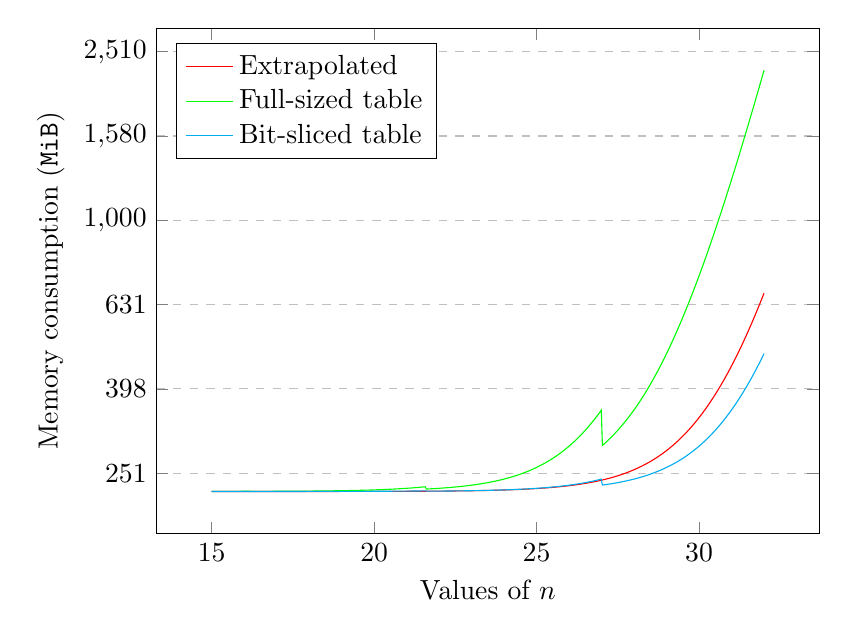
\begin{tikzpicture}
            \begin{axis}[
                xlabel=Values of $n$,
                ylabel=Memory consumption (\texttt{MiB}),
                ymode=log,
                legend cell align=left,
                log ticks with fixed point,
                xtick={15,20,25,30},
                height=8cm,
                width=10cm,
                ymajorgrids,
                grid style=dashed,
                legend pos=north west,
            ]
            \addplot[
                color=red,
                domain=15:32,
                samples=500,
            ]
            {(0.00013831083126693568 * 2^(0.988135062636788 * x) + 232634.0051135452)/1024};
            \addplot[
                color=green,
                domain=15:32,
                samples=500,
            ] {(4 * 8 * 2^(x - (ceil(x/5.4)))/1024 + 232634.0051135452)/1024};
            \addplot[
                color=cyan,
                domain=15:32,
                samples=500,
            ] {(4 * 2^(x - (ceil(x/5.4)))/1024 + 232634.0051135452)/1024};
            \legend{Extrapolated, Full-sized table, Bit-sliced table}
            \end{axis}
        \end{tikzpicture}
    \end{figure}
\end{frame}

\begin{frame}
    \frametitle{Memory: AVX and standard C implementations}
    \begin{figure}[t]
        \centering
        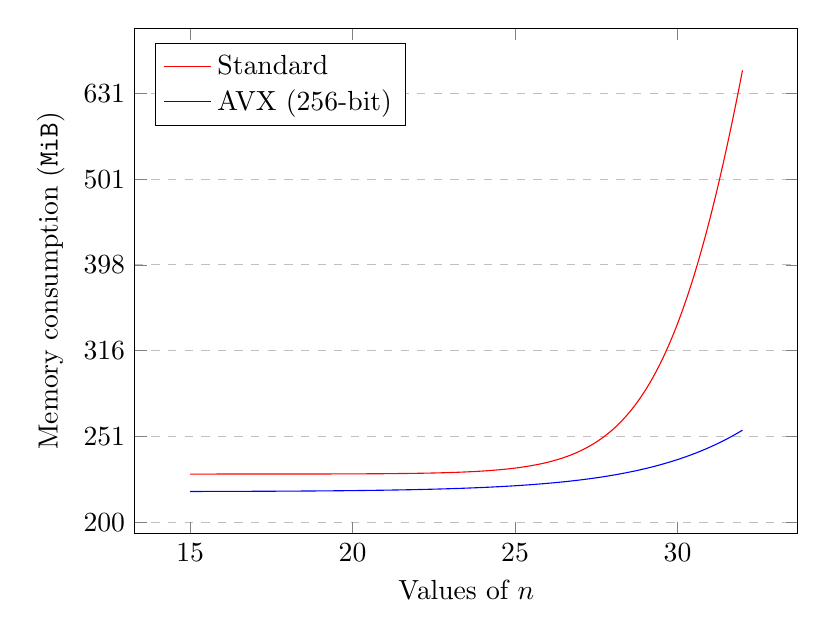
\begin{tikzpicture}
            \begin{axis}[
                xlabel=Values of $n$,
                ymode=log,
                legend cell align=left,
                log ticks with fixed point,
                ylabel=Memory consumption (\texttt{MiB}),
                xtick={15,20,25,30},
                height=8cm,
                width=10cm,
                ymajorgrids,
                grid style=dashed,
                legend pos=north west,
            ]
            \addplot[
                color=red,
                domain=15:32,
                samples=500,
            ]
            {(0.00013831083126693568 * 2^(0.988135062636788 * x) + 232634.0051135452)/1024};
            \addplot [
                color=blue,
                domain=15:32,
                samples=500,
            ] {(0.6300250132482776 * 2^(0.4984381599371818 * x) + 221906.00452997335)/1024};
            \legend{Standard, AVX (256-bit)}
            \end{axis}
        \end{tikzpicture}
    \end{figure}
\end{frame}

\begin{frame}
    \frametitle{Timings: Expectation}
    \begin{itemize}
        \item Both C variants outperform the simple FES implementation.
        \item The interpolation phase is bottlenecked FES-based recovery.
        \item Multicore scales well.
    \end{itemize}
\end{frame}

\begin{frame}
    \frametitle{Timings: Standard, AVX, and FES}
    \begin{figure}[t]
        \centering
        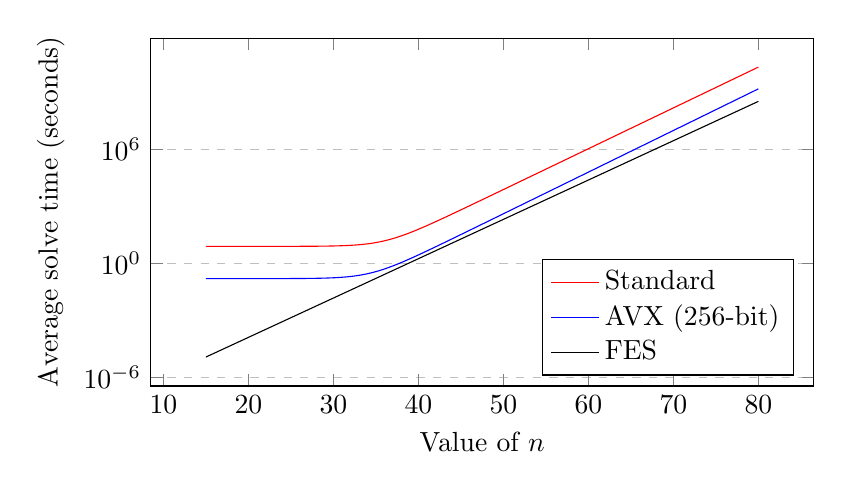
\begin{tikzpicture}
            \begin{axis}[
                xlabel={Value of $n$},
                ylabel={Average solve time (seconds)},
                legend cell align=left,
                ymode=log,
                ymajorgrids=true,
                grid style=dashed,
                height=6cm,
                width=10cm,
                legend pos=south east,
            ]
                \addplot [
                    color=red,
                    domain=15:80,
                    samples=500,
                ] {(0.00013821153801904347 * 2^(0.7131086234506752 * x) + 7680.492487663649)/1000};
                \addplot [
                    color=blue,
                    domain=15:80,
                    samples=500,
                ] {(4.515323644415954e-06 * 2^(0.7272699624665934 * x) + 154.55031285117195)/1000};
                \addplot [
                    color=black,
                    domain=15:80,
                    samples=500,
                ] {(9.23081156978058e-06 * 2^(0.6870633039068228 * x) + 5.026531141453392e-16)/1000};
                \legend{Standard, AVX (256-bit), FES} 
            \end{axis}
        \end{tikzpicture}
    \end{figure}
\end{frame}

\begin{frame}
    \frametitle{Timings: Breakdown}
    \begin{figure}[t]
        \centering
        %% Creator: Matplotlib, PGF backend
%%
%% To include the figure in your LaTeX document, write
%%   \input{<filename>.pgf}
%%
%% Make sure the required packages are loaded in your preamble
%%   \usepackage{pgf}
%%
%% Also ensure that all the required font packages are loaded; for instance,
%% the lmodern package is sometimes necessary when using math font.
%%   \usepackage{lmodern}
%%
%% Figures using additional raster images can only be included by \input if
%% they are in the same directory as the main LaTeX file. For loading figures
%% from other directories you can use the `import` package
%%   \usepackage{import}
%%
%% and then include the figures with
%%   \import{<path to file>}{<filename>.pgf}
%%
%% Matplotlib used the following preamble
%%   
%%   \usepackage{fontspec}
%%   \setmainfont{DejaVuSerif.ttf}[Path=\detokenize{/Users/moggel/Library/Python/3.9/lib/python/site-packages/matplotlib/mpl-data/fonts/ttf/}]
%%   \setsansfont{DejaVuSans.ttf}[Path=\detokenize{/Users/moggel/Library/Python/3.9/lib/python/site-packages/matplotlib/mpl-data/fonts/ttf/}]
%%   \setmonofont{DejaVuSansMono.ttf}[Path=\detokenize{/Users/moggel/Library/Python/3.9/lib/python/site-packages/matplotlib/mpl-data/fonts/ttf/}]
%%   \makeatletter\@ifpackageloaded{underscore}{}{\usepackage[strings]{underscore}}\makeatother
%%
\begingroup%
\makeatletter%
\begin{pgfpicture}%
\pgfpathrectangle{\pgfpointorigin}{\pgfqpoint{4.155577in}{2.566596in}}%
\pgfusepath{use as bounding box, clip}%
\begin{pgfscope}%
\pgfsetbuttcap%
\pgfsetmiterjoin%
\definecolor{currentfill}{rgb}{1.000000,1.000000,1.000000}%
\pgfsetfillcolor{currentfill}%
\pgfsetlinewidth{0.000000pt}%
\definecolor{currentstroke}{rgb}{1.000000,1.000000,1.000000}%
\pgfsetstrokecolor{currentstroke}%
\pgfsetdash{}{0pt}%
\pgfpathmoveto{\pgfqpoint{0.000000in}{0.000000in}}%
\pgfpathlineto{\pgfqpoint{4.155577in}{0.000000in}}%
\pgfpathlineto{\pgfqpoint{4.155577in}{2.566596in}}%
\pgfpathlineto{\pgfqpoint{0.000000in}{2.566596in}}%
\pgfpathlineto{\pgfqpoint{0.000000in}{0.000000in}}%
\pgfpathclose%
\pgfusepath{fill}%
\end{pgfscope}%
\begin{pgfscope}%
\pgfsetbuttcap%
\pgfsetmiterjoin%
\definecolor{currentfill}{rgb}{1.000000,1.000000,1.000000}%
\pgfsetfillcolor{currentfill}%
\pgfsetlinewidth{0.000000pt}%
\definecolor{currentstroke}{rgb}{0.000000,0.000000,0.000000}%
\pgfsetstrokecolor{currentstroke}%
\pgfsetstrokeopacity{0.000000}%
\pgfsetdash{}{0pt}%
\pgfpathmoveto{\pgfqpoint{0.563921in}{0.331635in}}%
\pgfpathlineto{\pgfqpoint{2.888921in}{0.331635in}}%
\pgfpathlineto{\pgfqpoint{2.888921in}{2.256635in}}%
\pgfpathlineto{\pgfqpoint{0.563921in}{2.256635in}}%
\pgfpathlineto{\pgfqpoint{0.563921in}{0.331635in}}%
\pgfpathclose%
\pgfusepath{fill}%
\end{pgfscope}%
\begin{pgfscope}%
\pgfpathrectangle{\pgfqpoint{0.563921in}{0.331635in}}{\pgfqpoint{2.325000in}{1.925000in}}%
\pgfusepath{clip}%
\pgfsetbuttcap%
\pgfsetmiterjoin%
\definecolor{currentfill}{rgb}{0.121569,0.466667,0.705882}%
\pgfsetfillcolor{currentfill}%
\pgfsetlinewidth{0.000000pt}%
\definecolor{currentstroke}{rgb}{0.000000,0.000000,0.000000}%
\pgfsetstrokecolor{currentstroke}%
\pgfsetstrokeopacity{0.000000}%
\pgfsetdash{}{0pt}%
\pgfpathmoveto{\pgfqpoint{0.563921in}{0.375385in}}%
\pgfpathlineto{\pgfqpoint{0.914745in}{0.375385in}}%
\pgfpathlineto{\pgfqpoint{0.914745in}{0.462885in}}%
\pgfpathlineto{\pgfqpoint{0.563921in}{0.462885in}}%
\pgfpathlineto{\pgfqpoint{0.563921in}{0.375385in}}%
\pgfpathclose%
\pgfusepath{fill}%
\end{pgfscope}%
\begin{pgfscope}%
\pgfpathrectangle{\pgfqpoint{0.563921in}{0.331635in}}{\pgfqpoint{2.325000in}{1.925000in}}%
\pgfusepath{clip}%
\pgfsetbuttcap%
\pgfsetmiterjoin%
\definecolor{currentfill}{rgb}{0.121569,0.466667,0.705882}%
\pgfsetfillcolor{currentfill}%
\pgfsetlinewidth{0.000000pt}%
\definecolor{currentstroke}{rgb}{0.000000,0.000000,0.000000}%
\pgfsetstrokecolor{currentstroke}%
\pgfsetstrokeopacity{0.000000}%
\pgfsetdash{}{0pt}%
\pgfpathmoveto{\pgfqpoint{0.563921in}{0.550385in}}%
\pgfpathlineto{\pgfqpoint{0.873557in}{0.550385in}}%
\pgfpathlineto{\pgfqpoint{0.873557in}{0.637885in}}%
\pgfpathlineto{\pgfqpoint{0.563921in}{0.637885in}}%
\pgfpathlineto{\pgfqpoint{0.563921in}{0.550385in}}%
\pgfpathclose%
\pgfusepath{fill}%
\end{pgfscope}%
\begin{pgfscope}%
\pgfpathrectangle{\pgfqpoint{0.563921in}{0.331635in}}{\pgfqpoint{2.325000in}{1.925000in}}%
\pgfusepath{clip}%
\pgfsetbuttcap%
\pgfsetmiterjoin%
\definecolor{currentfill}{rgb}{0.121569,0.466667,0.705882}%
\pgfsetfillcolor{currentfill}%
\pgfsetlinewidth{0.000000pt}%
\definecolor{currentstroke}{rgb}{0.000000,0.000000,0.000000}%
\pgfsetstrokecolor{currentstroke}%
\pgfsetstrokeopacity{0.000000}%
\pgfsetdash{}{0pt}%
\pgfpathmoveto{\pgfqpoint{0.563921in}{0.725385in}}%
\pgfpathlineto{\pgfqpoint{0.873835in}{0.725385in}}%
\pgfpathlineto{\pgfqpoint{0.873835in}{0.812885in}}%
\pgfpathlineto{\pgfqpoint{0.563921in}{0.812885in}}%
\pgfpathlineto{\pgfqpoint{0.563921in}{0.725385in}}%
\pgfpathclose%
\pgfusepath{fill}%
\end{pgfscope}%
\begin{pgfscope}%
\pgfpathrectangle{\pgfqpoint{0.563921in}{0.331635in}}{\pgfqpoint{2.325000in}{1.925000in}}%
\pgfusepath{clip}%
\pgfsetbuttcap%
\pgfsetmiterjoin%
\definecolor{currentfill}{rgb}{0.121569,0.466667,0.705882}%
\pgfsetfillcolor{currentfill}%
\pgfsetlinewidth{0.000000pt}%
\definecolor{currentstroke}{rgb}{0.000000,0.000000,0.000000}%
\pgfsetstrokecolor{currentstroke}%
\pgfsetstrokeopacity{0.000000}%
\pgfsetdash{}{0pt}%
\pgfpathmoveto{\pgfqpoint{0.563921in}{0.900385in}}%
\pgfpathlineto{\pgfqpoint{0.940195in}{0.900385in}}%
\pgfpathlineto{\pgfqpoint{0.940195in}{0.987885in}}%
\pgfpathlineto{\pgfqpoint{0.563921in}{0.987885in}}%
\pgfpathlineto{\pgfqpoint{0.563921in}{0.900385in}}%
\pgfpathclose%
\pgfusepath{fill}%
\end{pgfscope}%
\begin{pgfscope}%
\pgfpathrectangle{\pgfqpoint{0.563921in}{0.331635in}}{\pgfqpoint{2.325000in}{1.925000in}}%
\pgfusepath{clip}%
\pgfsetbuttcap%
\pgfsetmiterjoin%
\definecolor{currentfill}{rgb}{0.121569,0.466667,0.705882}%
\pgfsetfillcolor{currentfill}%
\pgfsetlinewidth{0.000000pt}%
\definecolor{currentstroke}{rgb}{0.000000,0.000000,0.000000}%
\pgfsetstrokecolor{currentstroke}%
\pgfsetstrokeopacity{0.000000}%
\pgfsetdash{}{0pt}%
\pgfpathmoveto{\pgfqpoint{0.563921in}{1.075385in}}%
\pgfpathlineto{\pgfqpoint{0.914663in}{1.075385in}}%
\pgfpathlineto{\pgfqpoint{0.914663in}{1.162885in}}%
\pgfpathlineto{\pgfqpoint{0.563921in}{1.162885in}}%
\pgfpathlineto{\pgfqpoint{0.563921in}{1.075385in}}%
\pgfpathclose%
\pgfusepath{fill}%
\end{pgfscope}%
\begin{pgfscope}%
\pgfpathrectangle{\pgfqpoint{0.563921in}{0.331635in}}{\pgfqpoint{2.325000in}{1.925000in}}%
\pgfusepath{clip}%
\pgfsetbuttcap%
\pgfsetmiterjoin%
\definecolor{currentfill}{rgb}{0.121569,0.466667,0.705882}%
\pgfsetfillcolor{currentfill}%
\pgfsetlinewidth{0.000000pt}%
\definecolor{currentstroke}{rgb}{0.000000,0.000000,0.000000}%
\pgfsetstrokecolor{currentstroke}%
\pgfsetstrokeopacity{0.000000}%
\pgfsetdash{}{0pt}%
\pgfpathmoveto{\pgfqpoint{0.563921in}{1.250385in}}%
\pgfpathlineto{\pgfqpoint{0.899737in}{1.250385in}}%
\pgfpathlineto{\pgfqpoint{0.899737in}{1.337885in}}%
\pgfpathlineto{\pgfqpoint{0.563921in}{1.337885in}}%
\pgfpathlineto{\pgfqpoint{0.563921in}{1.250385in}}%
\pgfpathclose%
\pgfusepath{fill}%
\end{pgfscope}%
\begin{pgfscope}%
\pgfpathrectangle{\pgfqpoint{0.563921in}{0.331635in}}{\pgfqpoint{2.325000in}{1.925000in}}%
\pgfusepath{clip}%
\pgfsetbuttcap%
\pgfsetmiterjoin%
\definecolor{currentfill}{rgb}{0.121569,0.466667,0.705882}%
\pgfsetfillcolor{currentfill}%
\pgfsetlinewidth{0.000000pt}%
\definecolor{currentstroke}{rgb}{0.000000,0.000000,0.000000}%
\pgfsetstrokecolor{currentstroke}%
\pgfsetstrokeopacity{0.000000}%
\pgfsetdash{}{0pt}%
\pgfpathmoveto{\pgfqpoint{0.563921in}{1.425385in}}%
\pgfpathlineto{\pgfqpoint{0.861305in}{1.425385in}}%
\pgfpathlineto{\pgfqpoint{0.861305in}{1.512885in}}%
\pgfpathlineto{\pgfqpoint{0.563921in}{1.512885in}}%
\pgfpathlineto{\pgfqpoint{0.563921in}{1.425385in}}%
\pgfpathclose%
\pgfusepath{fill}%
\end{pgfscope}%
\begin{pgfscope}%
\pgfpathrectangle{\pgfqpoint{0.563921in}{0.331635in}}{\pgfqpoint{2.325000in}{1.925000in}}%
\pgfusepath{clip}%
\pgfsetbuttcap%
\pgfsetmiterjoin%
\definecolor{currentfill}{rgb}{0.121569,0.466667,0.705882}%
\pgfsetfillcolor{currentfill}%
\pgfsetlinewidth{0.000000pt}%
\definecolor{currentstroke}{rgb}{0.000000,0.000000,0.000000}%
\pgfsetstrokecolor{currentstroke}%
\pgfsetstrokeopacity{0.000000}%
\pgfsetdash{}{0pt}%
\pgfpathmoveto{\pgfqpoint{0.563921in}{1.600385in}}%
\pgfpathlineto{\pgfqpoint{0.850476in}{1.600385in}}%
\pgfpathlineto{\pgfqpoint{0.850476in}{1.687885in}}%
\pgfpathlineto{\pgfqpoint{0.563921in}{1.687885in}}%
\pgfpathlineto{\pgfqpoint{0.563921in}{1.600385in}}%
\pgfpathclose%
\pgfusepath{fill}%
\end{pgfscope}%
\begin{pgfscope}%
\pgfpathrectangle{\pgfqpoint{0.563921in}{0.331635in}}{\pgfqpoint{2.325000in}{1.925000in}}%
\pgfusepath{clip}%
\pgfsetbuttcap%
\pgfsetmiterjoin%
\definecolor{currentfill}{rgb}{0.121569,0.466667,0.705882}%
\pgfsetfillcolor{currentfill}%
\pgfsetlinewidth{0.000000pt}%
\definecolor{currentstroke}{rgb}{0.000000,0.000000,0.000000}%
\pgfsetstrokecolor{currentstroke}%
\pgfsetstrokeopacity{0.000000}%
\pgfsetdash{}{0pt}%
\pgfpathmoveto{\pgfqpoint{0.563921in}{1.775385in}}%
\pgfpathlineto{\pgfqpoint{0.848953in}{1.775385in}}%
\pgfpathlineto{\pgfqpoint{0.848953in}{1.862885in}}%
\pgfpathlineto{\pgfqpoint{0.563921in}{1.862885in}}%
\pgfpathlineto{\pgfqpoint{0.563921in}{1.775385in}}%
\pgfpathclose%
\pgfusepath{fill}%
\end{pgfscope}%
\begin{pgfscope}%
\pgfpathrectangle{\pgfqpoint{0.563921in}{0.331635in}}{\pgfqpoint{2.325000in}{1.925000in}}%
\pgfusepath{clip}%
\pgfsetbuttcap%
\pgfsetmiterjoin%
\definecolor{currentfill}{rgb}{0.121569,0.466667,0.705882}%
\pgfsetfillcolor{currentfill}%
\pgfsetlinewidth{0.000000pt}%
\definecolor{currentstroke}{rgb}{0.000000,0.000000,0.000000}%
\pgfsetstrokecolor{currentstroke}%
\pgfsetstrokeopacity{0.000000}%
\pgfsetdash{}{0pt}%
\pgfpathmoveto{\pgfqpoint{0.563921in}{1.950385in}}%
\pgfpathlineto{\pgfqpoint{0.894626in}{1.950385in}}%
\pgfpathlineto{\pgfqpoint{0.894626in}{2.037885in}}%
\pgfpathlineto{\pgfqpoint{0.563921in}{2.037885in}}%
\pgfpathlineto{\pgfqpoint{0.563921in}{1.950385in}}%
\pgfpathclose%
\pgfusepath{fill}%
\end{pgfscope}%
\begin{pgfscope}%
\pgfpathrectangle{\pgfqpoint{0.563921in}{0.331635in}}{\pgfqpoint{2.325000in}{1.925000in}}%
\pgfusepath{clip}%
\pgfsetbuttcap%
\pgfsetmiterjoin%
\definecolor{currentfill}{rgb}{0.121569,0.466667,0.705882}%
\pgfsetfillcolor{currentfill}%
\pgfsetlinewidth{0.000000pt}%
\definecolor{currentstroke}{rgb}{0.000000,0.000000,0.000000}%
\pgfsetstrokecolor{currentstroke}%
\pgfsetstrokeopacity{0.000000}%
\pgfsetdash{}{0pt}%
\pgfpathmoveto{\pgfqpoint{0.563921in}{2.125385in}}%
\pgfpathlineto{\pgfqpoint{0.892031in}{2.125385in}}%
\pgfpathlineto{\pgfqpoint{0.892031in}{2.212885in}}%
\pgfpathlineto{\pgfqpoint{0.563921in}{2.212885in}}%
\pgfpathlineto{\pgfqpoint{0.563921in}{2.125385in}}%
\pgfpathclose%
\pgfusepath{fill}%
\end{pgfscope}%
\begin{pgfscope}%
\pgfpathrectangle{\pgfqpoint{0.563921in}{0.331635in}}{\pgfqpoint{2.325000in}{1.925000in}}%
\pgfusepath{clip}%
\pgfsetbuttcap%
\pgfsetmiterjoin%
\definecolor{currentfill}{rgb}{1.000000,0.498039,0.054902}%
\pgfsetfillcolor{currentfill}%
\pgfsetlinewidth{0.000000pt}%
\definecolor{currentstroke}{rgb}{0.000000,0.000000,0.000000}%
\pgfsetstrokecolor{currentstroke}%
\pgfsetstrokeopacity{0.000000}%
\pgfsetdash{}{0pt}%
\pgfpathmoveto{\pgfqpoint{0.914745in}{0.375385in}}%
\pgfpathlineto{\pgfqpoint{1.597180in}{0.375385in}}%
\pgfpathlineto{\pgfqpoint{1.597180in}{0.462885in}}%
\pgfpathlineto{\pgfqpoint{0.914745in}{0.462885in}}%
\pgfpathlineto{\pgfqpoint{0.914745in}{0.375385in}}%
\pgfpathclose%
\pgfusepath{fill}%
\end{pgfscope}%
\begin{pgfscope}%
\pgfpathrectangle{\pgfqpoint{0.563921in}{0.331635in}}{\pgfqpoint{2.325000in}{1.925000in}}%
\pgfusepath{clip}%
\pgfsetbuttcap%
\pgfsetmiterjoin%
\definecolor{currentfill}{rgb}{1.000000,0.498039,0.054902}%
\pgfsetfillcolor{currentfill}%
\pgfsetlinewidth{0.000000pt}%
\definecolor{currentstroke}{rgb}{0.000000,0.000000,0.000000}%
\pgfsetstrokecolor{currentstroke}%
\pgfsetstrokeopacity{0.000000}%
\pgfsetdash{}{0pt}%
\pgfpathmoveto{\pgfqpoint{0.873557in}{0.550385in}}%
\pgfpathlineto{\pgfqpoint{1.540571in}{0.550385in}}%
\pgfpathlineto{\pgfqpoint{1.540571in}{0.637885in}}%
\pgfpathlineto{\pgfqpoint{0.873557in}{0.637885in}}%
\pgfpathlineto{\pgfqpoint{0.873557in}{0.550385in}}%
\pgfpathclose%
\pgfusepath{fill}%
\end{pgfscope}%
\begin{pgfscope}%
\pgfpathrectangle{\pgfqpoint{0.563921in}{0.331635in}}{\pgfqpoint{2.325000in}{1.925000in}}%
\pgfusepath{clip}%
\pgfsetbuttcap%
\pgfsetmiterjoin%
\definecolor{currentfill}{rgb}{1.000000,0.498039,0.054902}%
\pgfsetfillcolor{currentfill}%
\pgfsetlinewidth{0.000000pt}%
\definecolor{currentstroke}{rgb}{0.000000,0.000000,0.000000}%
\pgfsetstrokecolor{currentstroke}%
\pgfsetstrokeopacity{0.000000}%
\pgfsetdash{}{0pt}%
\pgfpathmoveto{\pgfqpoint{0.873835in}{0.725385in}}%
\pgfpathlineto{\pgfqpoint{1.508747in}{0.725385in}}%
\pgfpathlineto{\pgfqpoint{1.508747in}{0.812885in}}%
\pgfpathlineto{\pgfqpoint{0.873835in}{0.812885in}}%
\pgfpathlineto{\pgfqpoint{0.873835in}{0.725385in}}%
\pgfpathclose%
\pgfusepath{fill}%
\end{pgfscope}%
\begin{pgfscope}%
\pgfpathrectangle{\pgfqpoint{0.563921in}{0.331635in}}{\pgfqpoint{2.325000in}{1.925000in}}%
\pgfusepath{clip}%
\pgfsetbuttcap%
\pgfsetmiterjoin%
\definecolor{currentfill}{rgb}{1.000000,0.498039,0.054902}%
\pgfsetfillcolor{currentfill}%
\pgfsetlinewidth{0.000000pt}%
\definecolor{currentstroke}{rgb}{0.000000,0.000000,0.000000}%
\pgfsetstrokecolor{currentstroke}%
\pgfsetstrokeopacity{0.000000}%
\pgfsetdash{}{0pt}%
\pgfpathmoveto{\pgfqpoint{0.940195in}{0.900385in}}%
\pgfpathlineto{\pgfqpoint{1.637200in}{0.900385in}}%
\pgfpathlineto{\pgfqpoint{1.637200in}{0.987885in}}%
\pgfpathlineto{\pgfqpoint{0.940195in}{0.987885in}}%
\pgfpathlineto{\pgfqpoint{0.940195in}{0.900385in}}%
\pgfpathclose%
\pgfusepath{fill}%
\end{pgfscope}%
\begin{pgfscope}%
\pgfpathrectangle{\pgfqpoint{0.563921in}{0.331635in}}{\pgfqpoint{2.325000in}{1.925000in}}%
\pgfusepath{clip}%
\pgfsetbuttcap%
\pgfsetmiterjoin%
\definecolor{currentfill}{rgb}{1.000000,0.498039,0.054902}%
\pgfsetfillcolor{currentfill}%
\pgfsetlinewidth{0.000000pt}%
\definecolor{currentstroke}{rgb}{0.000000,0.000000,0.000000}%
\pgfsetstrokecolor{currentstroke}%
\pgfsetstrokeopacity{0.000000}%
\pgfsetdash{}{0pt}%
\pgfpathmoveto{\pgfqpoint{0.914663in}{1.075385in}}%
\pgfpathlineto{\pgfqpoint{1.594545in}{1.075385in}}%
\pgfpathlineto{\pgfqpoint{1.594545in}{1.162885in}}%
\pgfpathlineto{\pgfqpoint{0.914663in}{1.162885in}}%
\pgfpathlineto{\pgfqpoint{0.914663in}{1.075385in}}%
\pgfpathclose%
\pgfusepath{fill}%
\end{pgfscope}%
\begin{pgfscope}%
\pgfpathrectangle{\pgfqpoint{0.563921in}{0.331635in}}{\pgfqpoint{2.325000in}{1.925000in}}%
\pgfusepath{clip}%
\pgfsetbuttcap%
\pgfsetmiterjoin%
\definecolor{currentfill}{rgb}{1.000000,0.498039,0.054902}%
\pgfsetfillcolor{currentfill}%
\pgfsetlinewidth{0.000000pt}%
\definecolor{currentstroke}{rgb}{0.000000,0.000000,0.000000}%
\pgfsetstrokecolor{currentstroke}%
\pgfsetstrokeopacity{0.000000}%
\pgfsetdash{}{0pt}%
\pgfpathmoveto{\pgfqpoint{0.899737in}{1.250385in}}%
\pgfpathlineto{\pgfqpoint{1.549794in}{1.250385in}}%
\pgfpathlineto{\pgfqpoint{1.549794in}{1.337885in}}%
\pgfpathlineto{\pgfqpoint{0.899737in}{1.337885in}}%
\pgfpathlineto{\pgfqpoint{0.899737in}{1.250385in}}%
\pgfpathclose%
\pgfusepath{fill}%
\end{pgfscope}%
\begin{pgfscope}%
\pgfpathrectangle{\pgfqpoint{0.563921in}{0.331635in}}{\pgfqpoint{2.325000in}{1.925000in}}%
\pgfusepath{clip}%
\pgfsetbuttcap%
\pgfsetmiterjoin%
\definecolor{currentfill}{rgb}{1.000000,0.498039,0.054902}%
\pgfsetfillcolor{currentfill}%
\pgfsetlinewidth{0.000000pt}%
\definecolor{currentstroke}{rgb}{0.000000,0.000000,0.000000}%
\pgfsetstrokecolor{currentstroke}%
\pgfsetstrokeopacity{0.000000}%
\pgfsetdash{}{0pt}%
\pgfpathmoveto{\pgfqpoint{0.861305in}{1.425385in}}%
\pgfpathlineto{\pgfqpoint{1.486197in}{1.425385in}}%
\pgfpathlineto{\pgfqpoint{1.486197in}{1.512885in}}%
\pgfpathlineto{\pgfqpoint{0.861305in}{1.512885in}}%
\pgfpathlineto{\pgfqpoint{0.861305in}{1.425385in}}%
\pgfpathclose%
\pgfusepath{fill}%
\end{pgfscope}%
\begin{pgfscope}%
\pgfpathrectangle{\pgfqpoint{0.563921in}{0.331635in}}{\pgfqpoint{2.325000in}{1.925000in}}%
\pgfusepath{clip}%
\pgfsetbuttcap%
\pgfsetmiterjoin%
\definecolor{currentfill}{rgb}{1.000000,0.498039,0.054902}%
\pgfsetfillcolor{currentfill}%
\pgfsetlinewidth{0.000000pt}%
\definecolor{currentstroke}{rgb}{0.000000,0.000000,0.000000}%
\pgfsetstrokecolor{currentstroke}%
\pgfsetstrokeopacity{0.000000}%
\pgfsetdash{}{0pt}%
\pgfpathmoveto{\pgfqpoint{0.850476in}{1.600385in}}%
\pgfpathlineto{\pgfqpoint{1.444899in}{1.600385in}}%
\pgfpathlineto{\pgfqpoint{1.444899in}{1.687885in}}%
\pgfpathlineto{\pgfqpoint{0.850476in}{1.687885in}}%
\pgfpathlineto{\pgfqpoint{0.850476in}{1.600385in}}%
\pgfpathclose%
\pgfusepath{fill}%
\end{pgfscope}%
\begin{pgfscope}%
\pgfpathrectangle{\pgfqpoint{0.563921in}{0.331635in}}{\pgfqpoint{2.325000in}{1.925000in}}%
\pgfusepath{clip}%
\pgfsetbuttcap%
\pgfsetmiterjoin%
\definecolor{currentfill}{rgb}{1.000000,0.498039,0.054902}%
\pgfsetfillcolor{currentfill}%
\pgfsetlinewidth{0.000000pt}%
\definecolor{currentstroke}{rgb}{0.000000,0.000000,0.000000}%
\pgfsetstrokecolor{currentstroke}%
\pgfsetstrokeopacity{0.000000}%
\pgfsetdash{}{0pt}%
\pgfpathmoveto{\pgfqpoint{0.848953in}{1.775385in}}%
\pgfpathlineto{\pgfqpoint{1.413943in}{1.775385in}}%
\pgfpathlineto{\pgfqpoint{1.413943in}{1.862885in}}%
\pgfpathlineto{\pgfqpoint{0.848953in}{1.862885in}}%
\pgfpathlineto{\pgfqpoint{0.848953in}{1.775385in}}%
\pgfpathclose%
\pgfusepath{fill}%
\end{pgfscope}%
\begin{pgfscope}%
\pgfpathrectangle{\pgfqpoint{0.563921in}{0.331635in}}{\pgfqpoint{2.325000in}{1.925000in}}%
\pgfusepath{clip}%
\pgfsetbuttcap%
\pgfsetmiterjoin%
\definecolor{currentfill}{rgb}{1.000000,0.498039,0.054902}%
\pgfsetfillcolor{currentfill}%
\pgfsetlinewidth{0.000000pt}%
\definecolor{currentstroke}{rgb}{0.000000,0.000000,0.000000}%
\pgfsetstrokecolor{currentstroke}%
\pgfsetstrokeopacity{0.000000}%
\pgfsetdash{}{0pt}%
\pgfpathmoveto{\pgfqpoint{0.894626in}{1.950385in}}%
\pgfpathlineto{\pgfqpoint{1.537550in}{1.950385in}}%
\pgfpathlineto{\pgfqpoint{1.537550in}{2.037885in}}%
\pgfpathlineto{\pgfqpoint{0.894626in}{2.037885in}}%
\pgfpathlineto{\pgfqpoint{0.894626in}{1.950385in}}%
\pgfpathclose%
\pgfusepath{fill}%
\end{pgfscope}%
\begin{pgfscope}%
\pgfpathrectangle{\pgfqpoint{0.563921in}{0.331635in}}{\pgfqpoint{2.325000in}{1.925000in}}%
\pgfusepath{clip}%
\pgfsetbuttcap%
\pgfsetmiterjoin%
\definecolor{currentfill}{rgb}{1.000000,0.498039,0.054902}%
\pgfsetfillcolor{currentfill}%
\pgfsetlinewidth{0.000000pt}%
\definecolor{currentstroke}{rgb}{0.000000,0.000000,0.000000}%
\pgfsetstrokecolor{currentstroke}%
\pgfsetstrokeopacity{0.000000}%
\pgfsetdash{}{0pt}%
\pgfpathmoveto{\pgfqpoint{0.892031in}{2.125385in}}%
\pgfpathlineto{\pgfqpoint{1.500593in}{2.125385in}}%
\pgfpathlineto{\pgfqpoint{1.500593in}{2.212885in}}%
\pgfpathlineto{\pgfqpoint{0.892031in}{2.212885in}}%
\pgfpathlineto{\pgfqpoint{0.892031in}{2.125385in}}%
\pgfpathclose%
\pgfusepath{fill}%
\end{pgfscope}%
\begin{pgfscope}%
\pgfpathrectangle{\pgfqpoint{0.563921in}{0.331635in}}{\pgfqpoint{2.325000in}{1.925000in}}%
\pgfusepath{clip}%
\pgfsetbuttcap%
\pgfsetmiterjoin%
\definecolor{currentfill}{rgb}{0.172549,0.627451,0.172549}%
\pgfsetfillcolor{currentfill}%
\pgfsetlinewidth{0.000000pt}%
\definecolor{currentstroke}{rgb}{0.000000,0.000000,0.000000}%
\pgfsetstrokecolor{currentstroke}%
\pgfsetstrokeopacity{0.000000}%
\pgfsetdash{}{0pt}%
\pgfpathmoveto{\pgfqpoint{1.597180in}{0.375385in}}%
\pgfpathlineto{\pgfqpoint{2.014493in}{0.375385in}}%
\pgfpathlineto{\pgfqpoint{2.014493in}{0.462885in}}%
\pgfpathlineto{\pgfqpoint{1.597180in}{0.462885in}}%
\pgfpathlineto{\pgfqpoint{1.597180in}{0.375385in}}%
\pgfpathclose%
\pgfusepath{fill}%
\end{pgfscope}%
\begin{pgfscope}%
\pgfpathrectangle{\pgfqpoint{0.563921in}{0.331635in}}{\pgfqpoint{2.325000in}{1.925000in}}%
\pgfusepath{clip}%
\pgfsetbuttcap%
\pgfsetmiterjoin%
\definecolor{currentfill}{rgb}{0.172549,0.627451,0.172549}%
\pgfsetfillcolor{currentfill}%
\pgfsetlinewidth{0.000000pt}%
\definecolor{currentstroke}{rgb}{0.000000,0.000000,0.000000}%
\pgfsetstrokecolor{currentstroke}%
\pgfsetstrokeopacity{0.000000}%
\pgfsetdash{}{0pt}%
\pgfpathmoveto{\pgfqpoint{1.540571in}{0.550385in}}%
\pgfpathlineto{\pgfqpoint{2.075168in}{0.550385in}}%
\pgfpathlineto{\pgfqpoint{2.075168in}{0.637885in}}%
\pgfpathlineto{\pgfqpoint{1.540571in}{0.637885in}}%
\pgfpathlineto{\pgfqpoint{1.540571in}{0.550385in}}%
\pgfpathclose%
\pgfusepath{fill}%
\end{pgfscope}%
\begin{pgfscope}%
\pgfpathrectangle{\pgfqpoint{0.563921in}{0.331635in}}{\pgfqpoint{2.325000in}{1.925000in}}%
\pgfusepath{clip}%
\pgfsetbuttcap%
\pgfsetmiterjoin%
\definecolor{currentfill}{rgb}{0.172549,0.627451,0.172549}%
\pgfsetfillcolor{currentfill}%
\pgfsetlinewidth{0.000000pt}%
\definecolor{currentstroke}{rgb}{0.000000,0.000000,0.000000}%
\pgfsetstrokecolor{currentstroke}%
\pgfsetstrokeopacity{0.000000}%
\pgfsetdash{}{0pt}%
\pgfpathmoveto{\pgfqpoint{1.508747in}{0.725385in}}%
\pgfpathlineto{\pgfqpoint{2.160766in}{0.725385in}}%
\pgfpathlineto{\pgfqpoint{2.160766in}{0.812885in}}%
\pgfpathlineto{\pgfqpoint{1.508747in}{0.812885in}}%
\pgfpathlineto{\pgfqpoint{1.508747in}{0.725385in}}%
\pgfpathclose%
\pgfusepath{fill}%
\end{pgfscope}%
\begin{pgfscope}%
\pgfpathrectangle{\pgfqpoint{0.563921in}{0.331635in}}{\pgfqpoint{2.325000in}{1.925000in}}%
\pgfusepath{clip}%
\pgfsetbuttcap%
\pgfsetmiterjoin%
\definecolor{currentfill}{rgb}{0.172549,0.627451,0.172549}%
\pgfsetfillcolor{currentfill}%
\pgfsetlinewidth{0.000000pt}%
\definecolor{currentstroke}{rgb}{0.000000,0.000000,0.000000}%
\pgfsetstrokecolor{currentstroke}%
\pgfsetstrokeopacity{0.000000}%
\pgfsetdash{}{0pt}%
\pgfpathmoveto{\pgfqpoint{1.637200in}{0.900385in}}%
\pgfpathlineto{\pgfqpoint{2.012794in}{0.900385in}}%
\pgfpathlineto{\pgfqpoint{2.012794in}{0.987885in}}%
\pgfpathlineto{\pgfqpoint{1.637200in}{0.987885in}}%
\pgfpathlineto{\pgfqpoint{1.637200in}{0.900385in}}%
\pgfpathclose%
\pgfusepath{fill}%
\end{pgfscope}%
\begin{pgfscope}%
\pgfpathrectangle{\pgfqpoint{0.563921in}{0.331635in}}{\pgfqpoint{2.325000in}{1.925000in}}%
\pgfusepath{clip}%
\pgfsetbuttcap%
\pgfsetmiterjoin%
\definecolor{currentfill}{rgb}{0.172549,0.627451,0.172549}%
\pgfsetfillcolor{currentfill}%
\pgfsetlinewidth{0.000000pt}%
\definecolor{currentstroke}{rgb}{0.000000,0.000000,0.000000}%
\pgfsetstrokecolor{currentstroke}%
\pgfsetstrokeopacity{0.000000}%
\pgfsetdash{}{0pt}%
\pgfpathmoveto{\pgfqpoint{1.594545in}{1.075385in}}%
\pgfpathlineto{\pgfqpoint{2.079523in}{1.075385in}}%
\pgfpathlineto{\pgfqpoint{2.079523in}{1.162885in}}%
\pgfpathlineto{\pgfqpoint{1.594545in}{1.162885in}}%
\pgfpathlineto{\pgfqpoint{1.594545in}{1.075385in}}%
\pgfpathclose%
\pgfusepath{fill}%
\end{pgfscope}%
\begin{pgfscope}%
\pgfpathrectangle{\pgfqpoint{0.563921in}{0.331635in}}{\pgfqpoint{2.325000in}{1.925000in}}%
\pgfusepath{clip}%
\pgfsetbuttcap%
\pgfsetmiterjoin%
\definecolor{currentfill}{rgb}{0.172549,0.627451,0.172549}%
\pgfsetfillcolor{currentfill}%
\pgfsetlinewidth{0.000000pt}%
\definecolor{currentstroke}{rgb}{0.000000,0.000000,0.000000}%
\pgfsetstrokecolor{currentstroke}%
\pgfsetstrokeopacity{0.000000}%
\pgfsetdash{}{0pt}%
\pgfpathmoveto{\pgfqpoint{1.549794in}{1.250385in}}%
\pgfpathlineto{\pgfqpoint{2.159075in}{1.250385in}}%
\pgfpathlineto{\pgfqpoint{2.159075in}{1.337885in}}%
\pgfpathlineto{\pgfqpoint{1.549794in}{1.337885in}}%
\pgfpathlineto{\pgfqpoint{1.549794in}{1.250385in}}%
\pgfpathclose%
\pgfusepath{fill}%
\end{pgfscope}%
\begin{pgfscope}%
\pgfpathrectangle{\pgfqpoint{0.563921in}{0.331635in}}{\pgfqpoint{2.325000in}{1.925000in}}%
\pgfusepath{clip}%
\pgfsetbuttcap%
\pgfsetmiterjoin%
\definecolor{currentfill}{rgb}{0.172549,0.627451,0.172549}%
\pgfsetfillcolor{currentfill}%
\pgfsetlinewidth{0.000000pt}%
\definecolor{currentstroke}{rgb}{0.000000,0.000000,0.000000}%
\pgfsetstrokecolor{currentstroke}%
\pgfsetstrokeopacity{0.000000}%
\pgfsetdash{}{0pt}%
\pgfpathmoveto{\pgfqpoint{1.486197in}{1.425385in}}%
\pgfpathlineto{\pgfqpoint{2.238797in}{1.425385in}}%
\pgfpathlineto{\pgfqpoint{2.238797in}{1.512885in}}%
\pgfpathlineto{\pgfqpoint{1.486197in}{1.512885in}}%
\pgfpathlineto{\pgfqpoint{1.486197in}{1.425385in}}%
\pgfpathclose%
\pgfusepath{fill}%
\end{pgfscope}%
\begin{pgfscope}%
\pgfpathrectangle{\pgfqpoint{0.563921in}{0.331635in}}{\pgfqpoint{2.325000in}{1.925000in}}%
\pgfusepath{clip}%
\pgfsetbuttcap%
\pgfsetmiterjoin%
\definecolor{currentfill}{rgb}{0.172549,0.627451,0.172549}%
\pgfsetfillcolor{currentfill}%
\pgfsetlinewidth{0.000000pt}%
\definecolor{currentstroke}{rgb}{0.000000,0.000000,0.000000}%
\pgfsetstrokecolor{currentstroke}%
\pgfsetstrokeopacity{0.000000}%
\pgfsetdash{}{0pt}%
\pgfpathmoveto{\pgfqpoint{1.444899in}{1.600385in}}%
\pgfpathlineto{\pgfqpoint{2.333574in}{1.600385in}}%
\pgfpathlineto{\pgfqpoint{2.333574in}{1.687885in}}%
\pgfpathlineto{\pgfqpoint{1.444899in}{1.687885in}}%
\pgfpathlineto{\pgfqpoint{1.444899in}{1.600385in}}%
\pgfpathclose%
\pgfusepath{fill}%
\end{pgfscope}%
\begin{pgfscope}%
\pgfpathrectangle{\pgfqpoint{0.563921in}{0.331635in}}{\pgfqpoint{2.325000in}{1.925000in}}%
\pgfusepath{clip}%
\pgfsetbuttcap%
\pgfsetmiterjoin%
\definecolor{currentfill}{rgb}{0.172549,0.627451,0.172549}%
\pgfsetfillcolor{currentfill}%
\pgfsetlinewidth{0.000000pt}%
\definecolor{currentstroke}{rgb}{0.000000,0.000000,0.000000}%
\pgfsetstrokecolor{currentstroke}%
\pgfsetstrokeopacity{0.000000}%
\pgfsetdash{}{0pt}%
\pgfpathmoveto{\pgfqpoint{1.413943in}{1.775385in}}%
\pgfpathlineto{\pgfqpoint{2.430586in}{1.775385in}}%
\pgfpathlineto{\pgfqpoint{2.430586in}{1.862885in}}%
\pgfpathlineto{\pgfqpoint{1.413943in}{1.862885in}}%
\pgfpathlineto{\pgfqpoint{1.413943in}{1.775385in}}%
\pgfpathclose%
\pgfusepath{fill}%
\end{pgfscope}%
\begin{pgfscope}%
\pgfpathrectangle{\pgfqpoint{0.563921in}{0.331635in}}{\pgfqpoint{2.325000in}{1.925000in}}%
\pgfusepath{clip}%
\pgfsetbuttcap%
\pgfsetmiterjoin%
\definecolor{currentfill}{rgb}{0.172549,0.627451,0.172549}%
\pgfsetfillcolor{currentfill}%
\pgfsetlinewidth{0.000000pt}%
\definecolor{currentstroke}{rgb}{0.000000,0.000000,0.000000}%
\pgfsetstrokecolor{currentstroke}%
\pgfsetstrokeopacity{0.000000}%
\pgfsetdash{}{0pt}%
\pgfpathmoveto{\pgfqpoint{1.537550in}{1.950385in}}%
\pgfpathlineto{\pgfqpoint{2.248257in}{1.950385in}}%
\pgfpathlineto{\pgfqpoint{2.248257in}{2.037885in}}%
\pgfpathlineto{\pgfqpoint{1.537550in}{2.037885in}}%
\pgfpathlineto{\pgfqpoint{1.537550in}{1.950385in}}%
\pgfpathclose%
\pgfusepath{fill}%
\end{pgfscope}%
\begin{pgfscope}%
\pgfpathrectangle{\pgfqpoint{0.563921in}{0.331635in}}{\pgfqpoint{2.325000in}{1.925000in}}%
\pgfusepath{clip}%
\pgfsetbuttcap%
\pgfsetmiterjoin%
\definecolor{currentfill}{rgb}{0.172549,0.627451,0.172549}%
\pgfsetfillcolor{currentfill}%
\pgfsetlinewidth{0.000000pt}%
\definecolor{currentstroke}{rgb}{0.000000,0.000000,0.000000}%
\pgfsetstrokecolor{currentstroke}%
\pgfsetstrokeopacity{0.000000}%
\pgfsetdash{}{0pt}%
\pgfpathmoveto{\pgfqpoint{1.500593in}{2.125385in}}%
\pgfpathlineto{\pgfqpoint{2.349281in}{2.125385in}}%
\pgfpathlineto{\pgfqpoint{2.349281in}{2.212885in}}%
\pgfpathlineto{\pgfqpoint{1.500593in}{2.212885in}}%
\pgfpathlineto{\pgfqpoint{1.500593in}{2.125385in}}%
\pgfpathclose%
\pgfusepath{fill}%
\end{pgfscope}%
\begin{pgfscope}%
\pgfpathrectangle{\pgfqpoint{0.563921in}{0.331635in}}{\pgfqpoint{2.325000in}{1.925000in}}%
\pgfusepath{clip}%
\pgfsetbuttcap%
\pgfsetmiterjoin%
\definecolor{currentfill}{rgb}{0.839216,0.152941,0.156863}%
\pgfsetfillcolor{currentfill}%
\pgfsetlinewidth{0.000000pt}%
\definecolor{currentstroke}{rgb}{0.000000,0.000000,0.000000}%
\pgfsetstrokecolor{currentstroke}%
\pgfsetstrokeopacity{0.000000}%
\pgfsetdash{}{0pt}%
\pgfpathmoveto{\pgfqpoint{2.014493in}{0.375385in}}%
\pgfpathlineto{\pgfqpoint{2.778207in}{0.375385in}}%
\pgfpathlineto{\pgfqpoint{2.778207in}{0.462885in}}%
\pgfpathlineto{\pgfqpoint{2.014493in}{0.462885in}}%
\pgfpathlineto{\pgfqpoint{2.014493in}{0.375385in}}%
\pgfpathclose%
\pgfusepath{fill}%
\end{pgfscope}%
\begin{pgfscope}%
\pgfpathrectangle{\pgfqpoint{0.563921in}{0.331635in}}{\pgfqpoint{2.325000in}{1.925000in}}%
\pgfusepath{clip}%
\pgfsetbuttcap%
\pgfsetmiterjoin%
\definecolor{currentfill}{rgb}{0.839216,0.152941,0.156863}%
\pgfsetfillcolor{currentfill}%
\pgfsetlinewidth{0.000000pt}%
\definecolor{currentstroke}{rgb}{0.000000,0.000000,0.000000}%
\pgfsetstrokecolor{currentstroke}%
\pgfsetstrokeopacity{0.000000}%
\pgfsetdash{}{0pt}%
\pgfpathmoveto{\pgfqpoint{2.075168in}{0.550385in}}%
\pgfpathlineto{\pgfqpoint{2.778207in}{0.550385in}}%
\pgfpathlineto{\pgfqpoint{2.778207in}{0.637885in}}%
\pgfpathlineto{\pgfqpoint{2.075168in}{0.637885in}}%
\pgfpathlineto{\pgfqpoint{2.075168in}{0.550385in}}%
\pgfpathclose%
\pgfusepath{fill}%
\end{pgfscope}%
\begin{pgfscope}%
\pgfpathrectangle{\pgfqpoint{0.563921in}{0.331635in}}{\pgfqpoint{2.325000in}{1.925000in}}%
\pgfusepath{clip}%
\pgfsetbuttcap%
\pgfsetmiterjoin%
\definecolor{currentfill}{rgb}{0.839216,0.152941,0.156863}%
\pgfsetfillcolor{currentfill}%
\pgfsetlinewidth{0.000000pt}%
\definecolor{currentstroke}{rgb}{0.000000,0.000000,0.000000}%
\pgfsetstrokecolor{currentstroke}%
\pgfsetstrokeopacity{0.000000}%
\pgfsetdash{}{0pt}%
\pgfpathmoveto{\pgfqpoint{2.160766in}{0.725385in}}%
\pgfpathlineto{\pgfqpoint{2.778207in}{0.725385in}}%
\pgfpathlineto{\pgfqpoint{2.778207in}{0.812885in}}%
\pgfpathlineto{\pgfqpoint{2.160766in}{0.812885in}}%
\pgfpathlineto{\pgfqpoint{2.160766in}{0.725385in}}%
\pgfpathclose%
\pgfusepath{fill}%
\end{pgfscope}%
\begin{pgfscope}%
\pgfpathrectangle{\pgfqpoint{0.563921in}{0.331635in}}{\pgfqpoint{2.325000in}{1.925000in}}%
\pgfusepath{clip}%
\pgfsetbuttcap%
\pgfsetmiterjoin%
\definecolor{currentfill}{rgb}{0.839216,0.152941,0.156863}%
\pgfsetfillcolor{currentfill}%
\pgfsetlinewidth{0.000000pt}%
\definecolor{currentstroke}{rgb}{0.000000,0.000000,0.000000}%
\pgfsetstrokecolor{currentstroke}%
\pgfsetstrokeopacity{0.000000}%
\pgfsetdash{}{0pt}%
\pgfpathmoveto{\pgfqpoint{2.012794in}{0.900385in}}%
\pgfpathlineto{\pgfqpoint{2.778207in}{0.900385in}}%
\pgfpathlineto{\pgfqpoint{2.778207in}{0.987885in}}%
\pgfpathlineto{\pgfqpoint{2.012794in}{0.987885in}}%
\pgfpathlineto{\pgfqpoint{2.012794in}{0.900385in}}%
\pgfpathclose%
\pgfusepath{fill}%
\end{pgfscope}%
\begin{pgfscope}%
\pgfpathrectangle{\pgfqpoint{0.563921in}{0.331635in}}{\pgfqpoint{2.325000in}{1.925000in}}%
\pgfusepath{clip}%
\pgfsetbuttcap%
\pgfsetmiterjoin%
\definecolor{currentfill}{rgb}{0.839216,0.152941,0.156863}%
\pgfsetfillcolor{currentfill}%
\pgfsetlinewidth{0.000000pt}%
\definecolor{currentstroke}{rgb}{0.000000,0.000000,0.000000}%
\pgfsetstrokecolor{currentstroke}%
\pgfsetstrokeopacity{0.000000}%
\pgfsetdash{}{0pt}%
\pgfpathmoveto{\pgfqpoint{2.079523in}{1.075385in}}%
\pgfpathlineto{\pgfqpoint{2.778207in}{1.075385in}}%
\pgfpathlineto{\pgfqpoint{2.778207in}{1.162885in}}%
\pgfpathlineto{\pgfqpoint{2.079523in}{1.162885in}}%
\pgfpathlineto{\pgfqpoint{2.079523in}{1.075385in}}%
\pgfpathclose%
\pgfusepath{fill}%
\end{pgfscope}%
\begin{pgfscope}%
\pgfpathrectangle{\pgfqpoint{0.563921in}{0.331635in}}{\pgfqpoint{2.325000in}{1.925000in}}%
\pgfusepath{clip}%
\pgfsetbuttcap%
\pgfsetmiterjoin%
\definecolor{currentfill}{rgb}{0.839216,0.152941,0.156863}%
\pgfsetfillcolor{currentfill}%
\pgfsetlinewidth{0.000000pt}%
\definecolor{currentstroke}{rgb}{0.000000,0.000000,0.000000}%
\pgfsetstrokecolor{currentstroke}%
\pgfsetstrokeopacity{0.000000}%
\pgfsetdash{}{0pt}%
\pgfpathmoveto{\pgfqpoint{2.159075in}{1.250385in}}%
\pgfpathlineto{\pgfqpoint{2.778207in}{1.250385in}}%
\pgfpathlineto{\pgfqpoint{2.778207in}{1.337885in}}%
\pgfpathlineto{\pgfqpoint{2.159075in}{1.337885in}}%
\pgfpathlineto{\pgfqpoint{2.159075in}{1.250385in}}%
\pgfpathclose%
\pgfusepath{fill}%
\end{pgfscope}%
\begin{pgfscope}%
\pgfpathrectangle{\pgfqpoint{0.563921in}{0.331635in}}{\pgfqpoint{2.325000in}{1.925000in}}%
\pgfusepath{clip}%
\pgfsetbuttcap%
\pgfsetmiterjoin%
\definecolor{currentfill}{rgb}{0.839216,0.152941,0.156863}%
\pgfsetfillcolor{currentfill}%
\pgfsetlinewidth{0.000000pt}%
\definecolor{currentstroke}{rgb}{0.000000,0.000000,0.000000}%
\pgfsetstrokecolor{currentstroke}%
\pgfsetstrokeopacity{0.000000}%
\pgfsetdash{}{0pt}%
\pgfpathmoveto{\pgfqpoint{2.238797in}{1.425385in}}%
\pgfpathlineto{\pgfqpoint{2.778207in}{1.425385in}}%
\pgfpathlineto{\pgfqpoint{2.778207in}{1.512885in}}%
\pgfpathlineto{\pgfqpoint{2.238797in}{1.512885in}}%
\pgfpathlineto{\pgfqpoint{2.238797in}{1.425385in}}%
\pgfpathclose%
\pgfusepath{fill}%
\end{pgfscope}%
\begin{pgfscope}%
\pgfpathrectangle{\pgfqpoint{0.563921in}{0.331635in}}{\pgfqpoint{2.325000in}{1.925000in}}%
\pgfusepath{clip}%
\pgfsetbuttcap%
\pgfsetmiterjoin%
\definecolor{currentfill}{rgb}{0.839216,0.152941,0.156863}%
\pgfsetfillcolor{currentfill}%
\pgfsetlinewidth{0.000000pt}%
\definecolor{currentstroke}{rgb}{0.000000,0.000000,0.000000}%
\pgfsetstrokecolor{currentstroke}%
\pgfsetstrokeopacity{0.000000}%
\pgfsetdash{}{0pt}%
\pgfpathmoveto{\pgfqpoint{2.333574in}{1.600385in}}%
\pgfpathlineto{\pgfqpoint{2.778207in}{1.600385in}}%
\pgfpathlineto{\pgfqpoint{2.778207in}{1.687885in}}%
\pgfpathlineto{\pgfqpoint{2.333574in}{1.687885in}}%
\pgfpathlineto{\pgfqpoint{2.333574in}{1.600385in}}%
\pgfpathclose%
\pgfusepath{fill}%
\end{pgfscope}%
\begin{pgfscope}%
\pgfpathrectangle{\pgfqpoint{0.563921in}{0.331635in}}{\pgfqpoint{2.325000in}{1.925000in}}%
\pgfusepath{clip}%
\pgfsetbuttcap%
\pgfsetmiterjoin%
\definecolor{currentfill}{rgb}{0.839216,0.152941,0.156863}%
\pgfsetfillcolor{currentfill}%
\pgfsetlinewidth{0.000000pt}%
\definecolor{currentstroke}{rgb}{0.000000,0.000000,0.000000}%
\pgfsetstrokecolor{currentstroke}%
\pgfsetstrokeopacity{0.000000}%
\pgfsetdash{}{0pt}%
\pgfpathmoveto{\pgfqpoint{2.430586in}{1.775385in}}%
\pgfpathlineto{\pgfqpoint{2.778207in}{1.775385in}}%
\pgfpathlineto{\pgfqpoint{2.778207in}{1.862885in}}%
\pgfpathlineto{\pgfqpoint{2.430586in}{1.862885in}}%
\pgfpathlineto{\pgfqpoint{2.430586in}{1.775385in}}%
\pgfpathclose%
\pgfusepath{fill}%
\end{pgfscope}%
\begin{pgfscope}%
\pgfpathrectangle{\pgfqpoint{0.563921in}{0.331635in}}{\pgfqpoint{2.325000in}{1.925000in}}%
\pgfusepath{clip}%
\pgfsetbuttcap%
\pgfsetmiterjoin%
\definecolor{currentfill}{rgb}{0.839216,0.152941,0.156863}%
\pgfsetfillcolor{currentfill}%
\pgfsetlinewidth{0.000000pt}%
\definecolor{currentstroke}{rgb}{0.000000,0.000000,0.000000}%
\pgfsetstrokecolor{currentstroke}%
\pgfsetstrokeopacity{0.000000}%
\pgfsetdash{}{0pt}%
\pgfpathmoveto{\pgfqpoint{2.248257in}{1.950385in}}%
\pgfpathlineto{\pgfqpoint{2.778207in}{1.950385in}}%
\pgfpathlineto{\pgfqpoint{2.778207in}{2.037885in}}%
\pgfpathlineto{\pgfqpoint{2.248257in}{2.037885in}}%
\pgfpathlineto{\pgfqpoint{2.248257in}{1.950385in}}%
\pgfpathclose%
\pgfusepath{fill}%
\end{pgfscope}%
\begin{pgfscope}%
\pgfpathrectangle{\pgfqpoint{0.563921in}{0.331635in}}{\pgfqpoint{2.325000in}{1.925000in}}%
\pgfusepath{clip}%
\pgfsetbuttcap%
\pgfsetmiterjoin%
\definecolor{currentfill}{rgb}{0.839216,0.152941,0.156863}%
\pgfsetfillcolor{currentfill}%
\pgfsetlinewidth{0.000000pt}%
\definecolor{currentstroke}{rgb}{0.000000,0.000000,0.000000}%
\pgfsetstrokecolor{currentstroke}%
\pgfsetstrokeopacity{0.000000}%
\pgfsetdash{}{0pt}%
\pgfpathmoveto{\pgfqpoint{2.349281in}{2.125385in}}%
\pgfpathlineto{\pgfqpoint{2.778207in}{2.125385in}}%
\pgfpathlineto{\pgfqpoint{2.778207in}{2.212885in}}%
\pgfpathlineto{\pgfqpoint{2.349281in}{2.212885in}}%
\pgfpathlineto{\pgfqpoint{2.349281in}{2.125385in}}%
\pgfpathclose%
\pgfusepath{fill}%
\end{pgfscope}%
\begin{pgfscope}%
\pgfsetbuttcap%
\pgfsetroundjoin%
\definecolor{currentfill}{rgb}{0.000000,0.000000,0.000000}%
\pgfsetfillcolor{currentfill}%
\pgfsetlinewidth{0.803000pt}%
\definecolor{currentstroke}{rgb}{0.000000,0.000000,0.000000}%
\pgfsetstrokecolor{currentstroke}%
\pgfsetdash{}{0pt}%
\pgfsys@defobject{currentmarker}{\pgfqpoint{0.000000in}{-0.048611in}}{\pgfqpoint{0.000000in}{0.000000in}}{%
\pgfpathmoveto{\pgfqpoint{0.000000in}{0.000000in}}%
\pgfpathlineto{\pgfqpoint{0.000000in}{-0.048611in}}%
\pgfusepath{stroke,fill}%
}%
\begin{pgfscope}%
\pgfsys@transformshift{0.563921in}{0.331635in}%
\pgfsys@useobject{currentmarker}{}%
\end{pgfscope}%
\end{pgfscope}%
\begin{pgfscope}%
\definecolor{textcolor}{rgb}{0.000000,0.000000,0.000000}%
\pgfsetstrokecolor{textcolor}%
\pgfsetfillcolor{textcolor}%
\pgftext[x=0.563921in,y=0.234413in,,top]{\color{textcolor}\sffamily\fontsize{10.000000}{12.000000}\selectfont 0}%
\end{pgfscope}%
\begin{pgfscope}%
\pgfsetbuttcap%
\pgfsetroundjoin%
\definecolor{currentfill}{rgb}{0.000000,0.000000,0.000000}%
\pgfsetfillcolor{currentfill}%
\pgfsetlinewidth{0.803000pt}%
\definecolor{currentstroke}{rgb}{0.000000,0.000000,0.000000}%
\pgfsetstrokecolor{currentstroke}%
\pgfsetdash{}{0pt}%
\pgfsys@defobject{currentmarker}{\pgfqpoint{0.000000in}{-0.048611in}}{\pgfqpoint{0.000000in}{0.000000in}}{%
\pgfpathmoveto{\pgfqpoint{0.000000in}{0.000000in}}%
\pgfpathlineto{\pgfqpoint{0.000000in}{-0.048611in}}%
\pgfusepath{stroke,fill}%
}%
\begin{pgfscope}%
\pgfsys@transformshift{1.117493in}{0.331635in}%
\pgfsys@useobject{currentmarker}{}%
\end{pgfscope}%
\end{pgfscope}%
\begin{pgfscope}%
\definecolor{textcolor}{rgb}{0.000000,0.000000,0.000000}%
\pgfsetstrokecolor{textcolor}%
\pgfsetfillcolor{textcolor}%
\pgftext[x=1.117493in,y=0.234413in,,top]{\color{textcolor}\sffamily\fontsize{10.000000}{12.000000}\selectfont 25}%
\end{pgfscope}%
\begin{pgfscope}%
\pgfsetbuttcap%
\pgfsetroundjoin%
\definecolor{currentfill}{rgb}{0.000000,0.000000,0.000000}%
\pgfsetfillcolor{currentfill}%
\pgfsetlinewidth{0.803000pt}%
\definecolor{currentstroke}{rgb}{0.000000,0.000000,0.000000}%
\pgfsetstrokecolor{currentstroke}%
\pgfsetdash{}{0pt}%
\pgfsys@defobject{currentmarker}{\pgfqpoint{0.000000in}{-0.048611in}}{\pgfqpoint{0.000000in}{0.000000in}}{%
\pgfpathmoveto{\pgfqpoint{0.000000in}{0.000000in}}%
\pgfpathlineto{\pgfqpoint{0.000000in}{-0.048611in}}%
\pgfusepath{stroke,fill}%
}%
\begin{pgfscope}%
\pgfsys@transformshift{1.671064in}{0.331635in}%
\pgfsys@useobject{currentmarker}{}%
\end{pgfscope}%
\end{pgfscope}%
\begin{pgfscope}%
\definecolor{textcolor}{rgb}{0.000000,0.000000,0.000000}%
\pgfsetstrokecolor{textcolor}%
\pgfsetfillcolor{textcolor}%
\pgftext[x=1.671064in,y=0.234413in,,top]{\color{textcolor}\sffamily\fontsize{10.000000}{12.000000}\selectfont 50}%
\end{pgfscope}%
\begin{pgfscope}%
\pgfsetbuttcap%
\pgfsetroundjoin%
\definecolor{currentfill}{rgb}{0.000000,0.000000,0.000000}%
\pgfsetfillcolor{currentfill}%
\pgfsetlinewidth{0.803000pt}%
\definecolor{currentstroke}{rgb}{0.000000,0.000000,0.000000}%
\pgfsetstrokecolor{currentstroke}%
\pgfsetdash{}{0pt}%
\pgfsys@defobject{currentmarker}{\pgfqpoint{0.000000in}{-0.048611in}}{\pgfqpoint{0.000000in}{0.000000in}}{%
\pgfpathmoveto{\pgfqpoint{0.000000in}{0.000000in}}%
\pgfpathlineto{\pgfqpoint{0.000000in}{-0.048611in}}%
\pgfusepath{stroke,fill}%
}%
\begin{pgfscope}%
\pgfsys@transformshift{2.224636in}{0.331635in}%
\pgfsys@useobject{currentmarker}{}%
\end{pgfscope}%
\end{pgfscope}%
\begin{pgfscope}%
\definecolor{textcolor}{rgb}{0.000000,0.000000,0.000000}%
\pgfsetstrokecolor{textcolor}%
\pgfsetfillcolor{textcolor}%
\pgftext[x=2.224636in,y=0.234413in,,top]{\color{textcolor}\sffamily\fontsize{10.000000}{12.000000}\selectfont 75}%
\end{pgfscope}%
\begin{pgfscope}%
\pgfsetbuttcap%
\pgfsetroundjoin%
\definecolor{currentfill}{rgb}{0.000000,0.000000,0.000000}%
\pgfsetfillcolor{currentfill}%
\pgfsetlinewidth{0.803000pt}%
\definecolor{currentstroke}{rgb}{0.000000,0.000000,0.000000}%
\pgfsetstrokecolor{currentstroke}%
\pgfsetdash{}{0pt}%
\pgfsys@defobject{currentmarker}{\pgfqpoint{0.000000in}{-0.048611in}}{\pgfqpoint{0.000000in}{0.000000in}}{%
\pgfpathmoveto{\pgfqpoint{0.000000in}{0.000000in}}%
\pgfpathlineto{\pgfqpoint{0.000000in}{-0.048611in}}%
\pgfusepath{stroke,fill}%
}%
\begin{pgfscope}%
\pgfsys@transformshift{2.778207in}{0.331635in}%
\pgfsys@useobject{currentmarker}{}%
\end{pgfscope}%
\end{pgfscope}%
\begin{pgfscope}%
\definecolor{textcolor}{rgb}{0.000000,0.000000,0.000000}%
\pgfsetstrokecolor{textcolor}%
\pgfsetfillcolor{textcolor}%
\pgftext[x=2.778207in,y=0.234413in,,top]{\color{textcolor}\sffamily\fontsize{10.000000}{12.000000}\selectfont 100}%
\end{pgfscope}%
\begin{pgfscope}%
\pgfsetbuttcap%
\pgfsetroundjoin%
\definecolor{currentfill}{rgb}{0.000000,0.000000,0.000000}%
\pgfsetfillcolor{currentfill}%
\pgfsetlinewidth{0.803000pt}%
\definecolor{currentstroke}{rgb}{0.000000,0.000000,0.000000}%
\pgfsetstrokecolor{currentstroke}%
\pgfsetdash{}{0pt}%
\pgfsys@defobject{currentmarker}{\pgfqpoint{-0.048611in}{0.000000in}}{\pgfqpoint{-0.000000in}{0.000000in}}{%
\pgfpathmoveto{\pgfqpoint{-0.000000in}{0.000000in}}%
\pgfpathlineto{\pgfqpoint{-0.048611in}{0.000000in}}%
\pgfusepath{stroke,fill}%
}%
\begin{pgfscope}%
\pgfsys@transformshift{0.563921in}{0.419135in}%
\pgfsys@useobject{currentmarker}{}%
\end{pgfscope}%
\end{pgfscope}%
\begin{pgfscope}%
\definecolor{textcolor}{rgb}{0.000000,0.000000,0.000000}%
\pgfsetstrokecolor{textcolor}%
\pgfsetfillcolor{textcolor}%
\pgftext[x=0.289968in, y=0.366373in, left, base]{\color{textcolor}\sffamily\fontsize{10.000000}{12.000000}\selectfont 30}%
\end{pgfscope}%
\begin{pgfscope}%
\pgfsetbuttcap%
\pgfsetroundjoin%
\definecolor{currentfill}{rgb}{0.000000,0.000000,0.000000}%
\pgfsetfillcolor{currentfill}%
\pgfsetlinewidth{0.803000pt}%
\definecolor{currentstroke}{rgb}{0.000000,0.000000,0.000000}%
\pgfsetstrokecolor{currentstroke}%
\pgfsetdash{}{0pt}%
\pgfsys@defobject{currentmarker}{\pgfqpoint{-0.048611in}{0.000000in}}{\pgfqpoint{-0.000000in}{0.000000in}}{%
\pgfpathmoveto{\pgfqpoint{-0.000000in}{0.000000in}}%
\pgfpathlineto{\pgfqpoint{-0.048611in}{0.000000in}}%
\pgfusepath{stroke,fill}%
}%
\begin{pgfscope}%
\pgfsys@transformshift{0.563921in}{0.594135in}%
\pgfsys@useobject{currentmarker}{}%
\end{pgfscope}%
\end{pgfscope}%
\begin{pgfscope}%
\definecolor{textcolor}{rgb}{0.000000,0.000000,0.000000}%
\pgfsetstrokecolor{textcolor}%
\pgfsetfillcolor{textcolor}%
\pgftext[x=0.289968in, y=0.541373in, left, base]{\color{textcolor}\sffamily\fontsize{10.000000}{12.000000}\selectfont 29}%
\end{pgfscope}%
\begin{pgfscope}%
\pgfsetbuttcap%
\pgfsetroundjoin%
\definecolor{currentfill}{rgb}{0.000000,0.000000,0.000000}%
\pgfsetfillcolor{currentfill}%
\pgfsetlinewidth{0.803000pt}%
\definecolor{currentstroke}{rgb}{0.000000,0.000000,0.000000}%
\pgfsetstrokecolor{currentstroke}%
\pgfsetdash{}{0pt}%
\pgfsys@defobject{currentmarker}{\pgfqpoint{-0.048611in}{0.000000in}}{\pgfqpoint{-0.000000in}{0.000000in}}{%
\pgfpathmoveto{\pgfqpoint{-0.000000in}{0.000000in}}%
\pgfpathlineto{\pgfqpoint{-0.048611in}{0.000000in}}%
\pgfusepath{stroke,fill}%
}%
\begin{pgfscope}%
\pgfsys@transformshift{0.563921in}{0.769135in}%
\pgfsys@useobject{currentmarker}{}%
\end{pgfscope}%
\end{pgfscope}%
\begin{pgfscope}%
\definecolor{textcolor}{rgb}{0.000000,0.000000,0.000000}%
\pgfsetstrokecolor{textcolor}%
\pgfsetfillcolor{textcolor}%
\pgftext[x=0.289968in, y=0.716373in, left, base]{\color{textcolor}\sffamily\fontsize{10.000000}{12.000000}\selectfont 28}%
\end{pgfscope}%
\begin{pgfscope}%
\pgfsetbuttcap%
\pgfsetroundjoin%
\definecolor{currentfill}{rgb}{0.000000,0.000000,0.000000}%
\pgfsetfillcolor{currentfill}%
\pgfsetlinewidth{0.803000pt}%
\definecolor{currentstroke}{rgb}{0.000000,0.000000,0.000000}%
\pgfsetstrokecolor{currentstroke}%
\pgfsetdash{}{0pt}%
\pgfsys@defobject{currentmarker}{\pgfqpoint{-0.048611in}{0.000000in}}{\pgfqpoint{-0.000000in}{0.000000in}}{%
\pgfpathmoveto{\pgfqpoint{-0.000000in}{0.000000in}}%
\pgfpathlineto{\pgfqpoint{-0.048611in}{0.000000in}}%
\pgfusepath{stroke,fill}%
}%
\begin{pgfscope}%
\pgfsys@transformshift{0.563921in}{0.944135in}%
\pgfsys@useobject{currentmarker}{}%
\end{pgfscope}%
\end{pgfscope}%
\begin{pgfscope}%
\definecolor{textcolor}{rgb}{0.000000,0.000000,0.000000}%
\pgfsetstrokecolor{textcolor}%
\pgfsetfillcolor{textcolor}%
\pgftext[x=0.289968in, y=0.891373in, left, base]{\color{textcolor}\sffamily\fontsize{10.000000}{12.000000}\selectfont 27}%
\end{pgfscope}%
\begin{pgfscope}%
\pgfsetbuttcap%
\pgfsetroundjoin%
\definecolor{currentfill}{rgb}{0.000000,0.000000,0.000000}%
\pgfsetfillcolor{currentfill}%
\pgfsetlinewidth{0.803000pt}%
\definecolor{currentstroke}{rgb}{0.000000,0.000000,0.000000}%
\pgfsetstrokecolor{currentstroke}%
\pgfsetdash{}{0pt}%
\pgfsys@defobject{currentmarker}{\pgfqpoint{-0.048611in}{0.000000in}}{\pgfqpoint{-0.000000in}{0.000000in}}{%
\pgfpathmoveto{\pgfqpoint{-0.000000in}{0.000000in}}%
\pgfpathlineto{\pgfqpoint{-0.048611in}{0.000000in}}%
\pgfusepath{stroke,fill}%
}%
\begin{pgfscope}%
\pgfsys@transformshift{0.563921in}{1.119135in}%
\pgfsys@useobject{currentmarker}{}%
\end{pgfscope}%
\end{pgfscope}%
\begin{pgfscope}%
\definecolor{textcolor}{rgb}{0.000000,0.000000,0.000000}%
\pgfsetstrokecolor{textcolor}%
\pgfsetfillcolor{textcolor}%
\pgftext[x=0.289968in, y=1.066373in, left, base]{\color{textcolor}\sffamily\fontsize{10.000000}{12.000000}\selectfont 26}%
\end{pgfscope}%
\begin{pgfscope}%
\pgfsetbuttcap%
\pgfsetroundjoin%
\definecolor{currentfill}{rgb}{0.000000,0.000000,0.000000}%
\pgfsetfillcolor{currentfill}%
\pgfsetlinewidth{0.803000pt}%
\definecolor{currentstroke}{rgb}{0.000000,0.000000,0.000000}%
\pgfsetstrokecolor{currentstroke}%
\pgfsetdash{}{0pt}%
\pgfsys@defobject{currentmarker}{\pgfqpoint{-0.048611in}{0.000000in}}{\pgfqpoint{-0.000000in}{0.000000in}}{%
\pgfpathmoveto{\pgfqpoint{-0.000000in}{0.000000in}}%
\pgfpathlineto{\pgfqpoint{-0.048611in}{0.000000in}}%
\pgfusepath{stroke,fill}%
}%
\begin{pgfscope}%
\pgfsys@transformshift{0.563921in}{1.294135in}%
\pgfsys@useobject{currentmarker}{}%
\end{pgfscope}%
\end{pgfscope}%
\begin{pgfscope}%
\definecolor{textcolor}{rgb}{0.000000,0.000000,0.000000}%
\pgfsetstrokecolor{textcolor}%
\pgfsetfillcolor{textcolor}%
\pgftext[x=0.289968in, y=1.241373in, left, base]{\color{textcolor}\sffamily\fontsize{10.000000}{12.000000}\selectfont 25}%
\end{pgfscope}%
\begin{pgfscope}%
\pgfsetbuttcap%
\pgfsetroundjoin%
\definecolor{currentfill}{rgb}{0.000000,0.000000,0.000000}%
\pgfsetfillcolor{currentfill}%
\pgfsetlinewidth{0.803000pt}%
\definecolor{currentstroke}{rgb}{0.000000,0.000000,0.000000}%
\pgfsetstrokecolor{currentstroke}%
\pgfsetdash{}{0pt}%
\pgfsys@defobject{currentmarker}{\pgfqpoint{-0.048611in}{0.000000in}}{\pgfqpoint{-0.000000in}{0.000000in}}{%
\pgfpathmoveto{\pgfqpoint{-0.000000in}{0.000000in}}%
\pgfpathlineto{\pgfqpoint{-0.048611in}{0.000000in}}%
\pgfusepath{stroke,fill}%
}%
\begin{pgfscope}%
\pgfsys@transformshift{0.563921in}{1.469135in}%
\pgfsys@useobject{currentmarker}{}%
\end{pgfscope}%
\end{pgfscope}%
\begin{pgfscope}%
\definecolor{textcolor}{rgb}{0.000000,0.000000,0.000000}%
\pgfsetstrokecolor{textcolor}%
\pgfsetfillcolor{textcolor}%
\pgftext[x=0.289968in, y=1.416373in, left, base]{\color{textcolor}\sffamily\fontsize{10.000000}{12.000000}\selectfont 24}%
\end{pgfscope}%
\begin{pgfscope}%
\pgfsetbuttcap%
\pgfsetroundjoin%
\definecolor{currentfill}{rgb}{0.000000,0.000000,0.000000}%
\pgfsetfillcolor{currentfill}%
\pgfsetlinewidth{0.803000pt}%
\definecolor{currentstroke}{rgb}{0.000000,0.000000,0.000000}%
\pgfsetstrokecolor{currentstroke}%
\pgfsetdash{}{0pt}%
\pgfsys@defobject{currentmarker}{\pgfqpoint{-0.048611in}{0.000000in}}{\pgfqpoint{-0.000000in}{0.000000in}}{%
\pgfpathmoveto{\pgfqpoint{-0.000000in}{0.000000in}}%
\pgfpathlineto{\pgfqpoint{-0.048611in}{0.000000in}}%
\pgfusepath{stroke,fill}%
}%
\begin{pgfscope}%
\pgfsys@transformshift{0.563921in}{1.644135in}%
\pgfsys@useobject{currentmarker}{}%
\end{pgfscope}%
\end{pgfscope}%
\begin{pgfscope}%
\definecolor{textcolor}{rgb}{0.000000,0.000000,0.000000}%
\pgfsetstrokecolor{textcolor}%
\pgfsetfillcolor{textcolor}%
\pgftext[x=0.289968in, y=1.591373in, left, base]{\color{textcolor}\sffamily\fontsize{10.000000}{12.000000}\selectfont 23}%
\end{pgfscope}%
\begin{pgfscope}%
\pgfsetbuttcap%
\pgfsetroundjoin%
\definecolor{currentfill}{rgb}{0.000000,0.000000,0.000000}%
\pgfsetfillcolor{currentfill}%
\pgfsetlinewidth{0.803000pt}%
\definecolor{currentstroke}{rgb}{0.000000,0.000000,0.000000}%
\pgfsetstrokecolor{currentstroke}%
\pgfsetdash{}{0pt}%
\pgfsys@defobject{currentmarker}{\pgfqpoint{-0.048611in}{0.000000in}}{\pgfqpoint{-0.000000in}{0.000000in}}{%
\pgfpathmoveto{\pgfqpoint{-0.000000in}{0.000000in}}%
\pgfpathlineto{\pgfqpoint{-0.048611in}{0.000000in}}%
\pgfusepath{stroke,fill}%
}%
\begin{pgfscope}%
\pgfsys@transformshift{0.563921in}{1.819135in}%
\pgfsys@useobject{currentmarker}{}%
\end{pgfscope}%
\end{pgfscope}%
\begin{pgfscope}%
\definecolor{textcolor}{rgb}{0.000000,0.000000,0.000000}%
\pgfsetstrokecolor{textcolor}%
\pgfsetfillcolor{textcolor}%
\pgftext[x=0.289968in, y=1.766373in, left, base]{\color{textcolor}\sffamily\fontsize{10.000000}{12.000000}\selectfont 22}%
\end{pgfscope}%
\begin{pgfscope}%
\pgfsetbuttcap%
\pgfsetroundjoin%
\definecolor{currentfill}{rgb}{0.000000,0.000000,0.000000}%
\pgfsetfillcolor{currentfill}%
\pgfsetlinewidth{0.803000pt}%
\definecolor{currentstroke}{rgb}{0.000000,0.000000,0.000000}%
\pgfsetstrokecolor{currentstroke}%
\pgfsetdash{}{0pt}%
\pgfsys@defobject{currentmarker}{\pgfqpoint{-0.048611in}{0.000000in}}{\pgfqpoint{-0.000000in}{0.000000in}}{%
\pgfpathmoveto{\pgfqpoint{-0.000000in}{0.000000in}}%
\pgfpathlineto{\pgfqpoint{-0.048611in}{0.000000in}}%
\pgfusepath{stroke,fill}%
}%
\begin{pgfscope}%
\pgfsys@transformshift{0.563921in}{1.994135in}%
\pgfsys@useobject{currentmarker}{}%
\end{pgfscope}%
\end{pgfscope}%
\begin{pgfscope}%
\definecolor{textcolor}{rgb}{0.000000,0.000000,0.000000}%
\pgfsetstrokecolor{textcolor}%
\pgfsetfillcolor{textcolor}%
\pgftext[x=0.289968in, y=1.941373in, left, base]{\color{textcolor}\sffamily\fontsize{10.000000}{12.000000}\selectfont 21}%
\end{pgfscope}%
\begin{pgfscope}%
\pgfsetbuttcap%
\pgfsetroundjoin%
\definecolor{currentfill}{rgb}{0.000000,0.000000,0.000000}%
\pgfsetfillcolor{currentfill}%
\pgfsetlinewidth{0.803000pt}%
\definecolor{currentstroke}{rgb}{0.000000,0.000000,0.000000}%
\pgfsetstrokecolor{currentstroke}%
\pgfsetdash{}{0pt}%
\pgfsys@defobject{currentmarker}{\pgfqpoint{-0.048611in}{0.000000in}}{\pgfqpoint{-0.000000in}{0.000000in}}{%
\pgfpathmoveto{\pgfqpoint{-0.000000in}{0.000000in}}%
\pgfpathlineto{\pgfqpoint{-0.048611in}{0.000000in}}%
\pgfusepath{stroke,fill}%
}%
\begin{pgfscope}%
\pgfsys@transformshift{0.563921in}{2.169135in}%
\pgfsys@useobject{currentmarker}{}%
\end{pgfscope}%
\end{pgfscope}%
\begin{pgfscope}%
\definecolor{textcolor}{rgb}{0.000000,0.000000,0.000000}%
\pgfsetstrokecolor{textcolor}%
\pgfsetfillcolor{textcolor}%
\pgftext[x=0.289968in, y=2.116373in, left, base]{\color{textcolor}\sffamily\fontsize{10.000000}{12.000000}\selectfont 20}%
\end{pgfscope}%
\begin{pgfscope}%
\definecolor{textcolor}{rgb}{0.000000,0.000000,0.000000}%
\pgfsetstrokecolor{textcolor}%
\pgfsetfillcolor{textcolor}%
\pgftext[x=0.234413in,y=1.294135in,,bottom,rotate=90.000000]{\color{textcolor}\sffamily\fontsize{10.000000}{12.000000}\selectfont \(\displaystyle n\)}%
\end{pgfscope}%
\begin{pgfscope}%
\pgfsetrectcap%
\pgfsetmiterjoin%
\pgfsetlinewidth{0.803000pt}%
\definecolor{currentstroke}{rgb}{0.000000,0.000000,0.000000}%
\pgfsetstrokecolor{currentstroke}%
\pgfsetdash{}{0pt}%
\pgfpathmoveto{\pgfqpoint{0.563921in}{0.331635in}}%
\pgfpathlineto{\pgfqpoint{0.563921in}{2.256635in}}%
\pgfusepath{stroke}%
\end{pgfscope}%
\begin{pgfscope}%
\pgfsetrectcap%
\pgfsetmiterjoin%
\pgfsetlinewidth{0.803000pt}%
\definecolor{currentstroke}{rgb}{0.000000,0.000000,0.000000}%
\pgfsetstrokecolor{currentstroke}%
\pgfsetdash{}{0pt}%
\pgfpathmoveto{\pgfqpoint{2.888921in}{0.331635in}}%
\pgfpathlineto{\pgfqpoint{2.888921in}{2.256635in}}%
\pgfusepath{stroke}%
\end{pgfscope}%
\begin{pgfscope}%
\pgfsetrectcap%
\pgfsetmiterjoin%
\pgfsetlinewidth{0.803000pt}%
\definecolor{currentstroke}{rgb}{0.000000,0.000000,0.000000}%
\pgfsetstrokecolor{currentstroke}%
\pgfsetdash{}{0pt}%
\pgfpathmoveto{\pgfqpoint{0.563921in}{0.331635in}}%
\pgfpathlineto{\pgfqpoint{2.888921in}{0.331635in}}%
\pgfusepath{stroke}%
\end{pgfscope}%
\begin{pgfscope}%
\pgfsetrectcap%
\pgfsetmiterjoin%
\pgfsetlinewidth{0.803000pt}%
\definecolor{currentstroke}{rgb}{0.000000,0.000000,0.000000}%
\pgfsetstrokecolor{currentstroke}%
\pgfsetdash{}{0pt}%
\pgfpathmoveto{\pgfqpoint{0.563921in}{2.256635in}}%
\pgfpathlineto{\pgfqpoint{2.888921in}{2.256635in}}%
\pgfusepath{stroke}%
\end{pgfscope}%
\begin{pgfscope}%
\definecolor{textcolor}{rgb}{0.000000,0.000000,0.000000}%
\pgfsetstrokecolor{textcolor}%
\pgfsetfillcolor{textcolor}%
\pgftext[x=1.726421in,y=2.339968in,,base]{\color{textcolor}\sffamily\fontsize{12.000000}{14.400000}\selectfont Breakdown of Solve times (\%)}%
\end{pgfscope}%
\begin{pgfscope}%
\pgfsetbuttcap%
\pgfsetmiterjoin%
\definecolor{currentfill}{rgb}{1.000000,1.000000,1.000000}%
\pgfsetfillcolor{currentfill}%
\pgfsetfillopacity{0.800000}%
\pgfsetlinewidth{1.003750pt}%
\definecolor{currentstroke}{rgb}{0.000000,0.000000,0.000000}%
\pgfsetstrokecolor{currentstroke}%
\pgfsetstrokeopacity{0.800000}%
\pgfsetdash{}{0pt}%
\pgfpathmoveto{\pgfqpoint{2.911143in}{1.501319in}}%
\pgfpathlineto{\pgfqpoint{4.088910in}{1.501319in}}%
\pgfpathlineto{\pgfqpoint{4.088910in}{2.253663in}}%
\pgfpathlineto{\pgfqpoint{2.911143in}{2.253663in}}%
\pgfpathlineto{\pgfqpoint{2.911143in}{1.501319in}}%
\pgfpathclose%
\pgfusepath{stroke,fill}%
\end{pgfscope}%
\begin{pgfscope}%
\pgfsetbuttcap%
\pgfsetmiterjoin%
\definecolor{currentfill}{rgb}{0.121569,0.466667,0.705882}%
\pgfsetfillcolor{currentfill}%
\pgfsetlinewidth{0.000000pt}%
\definecolor{currentstroke}{rgb}{0.000000,0.000000,0.000000}%
\pgfsetstrokecolor{currentstroke}%
\pgfsetstrokeopacity{0.000000}%
\pgfsetdash{}{0pt}%
\pgfpathmoveto{\pgfqpoint{2.988921in}{2.091467in}}%
\pgfpathlineto{\pgfqpoint{3.211143in}{2.091467in}}%
\pgfpathlineto{\pgfqpoint{3.211143in}{2.169244in}}%
\pgfpathlineto{\pgfqpoint{2.988921in}{2.169244in}}%
\pgfpathlineto{\pgfqpoint{2.988921in}{2.091467in}}%
\pgfpathclose%
\pgfusepath{fill}%
\end{pgfscope}%
\begin{pgfscope}%
\definecolor{textcolor}{rgb}{0.000000,0.000000,0.000000}%
\pgfsetstrokecolor{textcolor}%
\pgfsetfillcolor{textcolor}%
\pgftext[x=3.300032in,y=2.091467in,left,base]{\color{textcolor}\sffamily\fontsize{8.000000}{9.600000}\selectfont Total}%
\end{pgfscope}%
\begin{pgfscope}%
\pgfsetbuttcap%
\pgfsetmiterjoin%
\definecolor{currentfill}{rgb}{1.000000,0.498039,0.054902}%
\pgfsetfillcolor{currentfill}%
\pgfsetlinewidth{0.000000pt}%
\definecolor{currentstroke}{rgb}{0.000000,0.000000,0.000000}%
\pgfsetstrokecolor{currentstroke}%
\pgfsetstrokeopacity{0.000000}%
\pgfsetdash{}{0pt}%
\pgfpathmoveto{\pgfqpoint{2.988921in}{1.928381in}}%
\pgfpathlineto{\pgfqpoint{3.211143in}{1.928381in}}%
\pgfpathlineto{\pgfqpoint{3.211143in}{2.006158in}}%
\pgfpathlineto{\pgfqpoint{2.988921in}{2.006158in}}%
\pgfpathlineto{\pgfqpoint{2.988921in}{1.928381in}}%
\pgfpathclose%
\pgfusepath{fill}%
\end{pgfscope}%
\begin{pgfscope}%
\definecolor{textcolor}{rgb}{0.000000,0.000000,0.000000}%
\pgfsetstrokecolor{textcolor}%
\pgfsetfillcolor{textcolor}%
\pgftext[x=3.300032in,y=1.928381in,left,base]{\color{textcolor}\sffamily\fontsize{8.000000}{9.600000}\selectfont Recovery}%
\end{pgfscope}%
\begin{pgfscope}%
\pgfsetbuttcap%
\pgfsetmiterjoin%
\definecolor{currentfill}{rgb}{0.172549,0.627451,0.172549}%
\pgfsetfillcolor{currentfill}%
\pgfsetlinewidth{0.000000pt}%
\definecolor{currentstroke}{rgb}{0.000000,0.000000,0.000000}%
\pgfsetstrokecolor{currentstroke}%
\pgfsetstrokeopacity{0.000000}%
\pgfsetdash{}{0pt}%
\pgfpathmoveto{\pgfqpoint{2.988921in}{1.765295in}}%
\pgfpathlineto{\pgfqpoint{3.211143in}{1.765295in}}%
\pgfpathlineto{\pgfqpoint{3.211143in}{1.843073in}}%
\pgfpathlineto{\pgfqpoint{2.988921in}{1.843073in}}%
\pgfpathlineto{\pgfqpoint{2.988921in}{1.765295in}}%
\pgfpathclose%
\pgfusepath{fill}%
\end{pgfscope}%
\begin{pgfscope}%
\definecolor{textcolor}{rgb}{0.000000,0.000000,0.000000}%
\pgfsetstrokecolor{textcolor}%
\pgfsetfillcolor{textcolor}%
\pgftext[x=3.300032in,y=1.765295in,left,base]{\color{textcolor}\sffamily\fontsize{8.000000}{9.600000}\selectfont Interpolation}%
\end{pgfscope}%
\begin{pgfscope}%
\pgfsetbuttcap%
\pgfsetmiterjoin%
\definecolor{currentfill}{rgb}{0.839216,0.152941,0.156863}%
\pgfsetfillcolor{currentfill}%
\pgfsetlinewidth{0.000000pt}%
\definecolor{currentstroke}{rgb}{0.000000,0.000000,0.000000}%
\pgfsetstrokecolor{currentstroke}%
\pgfsetstrokeopacity{0.000000}%
\pgfsetdash{}{0pt}%
\pgfpathmoveto{\pgfqpoint{2.988921in}{1.602209in}}%
\pgfpathlineto{\pgfqpoint{3.211143in}{1.602209in}}%
\pgfpathlineto{\pgfqpoint{3.211143in}{1.679987in}}%
\pgfpathlineto{\pgfqpoint{2.988921in}{1.679987in}}%
\pgfpathlineto{\pgfqpoint{2.988921in}{1.602209in}}%
\pgfpathclose%
\pgfusepath{fill}%
\end{pgfscope}%
\begin{pgfscope}%
\definecolor{textcolor}{rgb}{0.000000,0.000000,0.000000}%
\pgfsetstrokecolor{textcolor}%
\pgfsetfillcolor{textcolor}%
\pgftext[x=3.300032in,y=1.602209in,left,base]{\color{textcolor}\sffamily\fontsize{8.000000}{9.600000}\selectfont Evaluation}%
\end{pgfscope}%
\end{pgfpicture}%
\makeatother%
\endgroup%

    \end{figure}
\end{frame}

\begin{frame}
    \frametitle{Conclusion}
    \begin{outline}
        \1 Provided an extendable practical implementation of Dinur's polynomial-method solver.
            \2 Three implementations:
                \3 SageMath prototyping.
                \3 Less optimized C implementation.
                \3 AVX optimized C implementation.
        \1 Benchmarks on the practical performance of the algorithm.
        \1 Introduction of polynomial interpolation using the principles of the FES procedure.
    \end{outline}
\end{frame}

\begin{frame}
    \frametitle{Future work}
    Examples:
    \begin{itemize}
        \item Find the problem with the number of potential solutions.
        \item Check impact of $n_1$.
        \item Proper Möbius transform setup.
        \item Further multicore and AVX support.
        \item Loop unrolling.
        \item Variable fixation.
    \end{itemize}
\end{frame}

\begin{frame}
    \frametitle{References}
    \printbibliography
\end{frame}

\section{Appendix}

\begin{frame}
    \frametitle{Appendix: Standard, AVX, and FES timings}
    \begin{table}[t]
        \begin{center}
            \pgfplotstabletypeset[
                col sep=comma,
                columns={standard,vectorized,fes,n},
                columns/standard/.style={
                    column name=Standard,
                    postproc cell content/.append style={
                        /pgfplots/table/@cell content/.add={}{ ms}
                    },
                },
                columns/vectorized/.style={
                    column name=Vectorized,
                    postproc cell content/.append style={
                            /pgfplots/table/@cell content/.add={}{ ms}
                    },
                },
                columns/fes/.style={
                    column name=FES,
                    postproc cell content/.append style={
                        /pgfplots/table/@cell content/.add={}{ ms},
                    },
                },
                columns/n/.style={
                    column name={$n,m$},
                },   
                every even row/.style={
                    before row={
                      \rowcolor[gray]{0.9}
                    }
                },
                every head row/.style={
                    before row=\toprule,
                    after row=\midrule
                },
                every last row/.style={
                    after row=\bottomrule
                },
           ]{metrics/fes_dinur/bench_comp.csv}
        \end{center}
    \end{table}
\end{frame}

\begin{frame}
    \frametitle{Appendix: FES-recovery timings for standard C implementation}
    \begin{table}[t]
        \begin{center}
            \pgfplotstabletypeset[
                col sep=comma,
                columns={recovery,interpolation,evaluation,n},
                columns/recovery/.style={
                    column name=Recovery,
                    postproc cell content/.append style={
                        /pgfplots/table/@cell content/.add={}{ ms}
                    },
                },
                columns/interpolation/.style={
                    column name=Interpolation,
                    postproc cell content/.append style={
                            /pgfplots/table/@cell content/.add={}{ ms}
                    },
                },
                columns/evaluation/.style={
                    column name=Evaluation,
                    postproc cell content/.append style={
                        /pgfplots/table/@cell content/.add={}{ ms},
                    },
                },
                columns/n/.style={
                    column name={$n,m$},
                },   
                every even row/.style={
                    before row={
                      \rowcolor[gray]{0.9}
                    }
                },
                every head row/.style={
                    before row=\toprule,
                    after row=\midrule
                },
                every last row/.style={
                    after row=\bottomrule
                },
           ]{metrics/fes_dinur/bench_recover.csv}
        \end{center}
    \end{table}
\end{frame}

\begin{frame}
    \frametitle{Appendix: $U$ polynomials}
    \begin{equation*}
        \begin{split}
            U_0(\mathbf{y}) &= \sum_{\hat{\mathbf{z}} \in \{0,1\}^{n_1}} \Tilde{F}(\mathbf{y},\hat{\mathbf{z}}),\\
            U_i(\mathbf{y}) &= \sum_{\hat{\mathbf{z}}\in \{0,1\}^{n_1 - 1}} \Tilde{F}_{z_{i - 1} \leftarrow 0}(\mathbf{y}, \hat{\mathbf{z}}), \text{ for } i = 1, \dots n_1.
        \end{split}
    \end{equation*}
\end{frame}

\begin{frame}
    \frametitle{Appendix: Regression explainability}
    \begin{itemize}
        \item[] Standard C (Memory): $R^2 = 0.9883$
        \vspace{0.5cm}
        \item[] AVX C (Memory): $R^2 = 0.9828$
        \vspace{0.5cm}
        \item[] Standard C (Timings): $R^2 = 0.9727$
        \vspace{0.5cm}
        \item[] AVX C (Timings): $R^2 = 0.9962$
        \vspace{0.5cm}
        \item[] FES (Timings): $R^2 = 1.0000$
    \end{itemize}
\end{frame}

\end{document}